\documentclass[
  10pt,
  aspectratio=169,   % 16:9 Widescreen
  %handout           % Uncomment for handout mode (no overlays)
]{beamer}

% ==============================
% Encoding & Fonts
% ==============================
\usepackage[T1]{fontenc}
\usepackage{tgheros}         % Sans-serif text font
\usepackage{newpxmath}       % Palatino-like math font
\usefonttheme{professionalfonts}
\usepackage{fix-cm}          % Flexible font sizes
\usepackage{bm}              % Bold math

% ==============================
% Theorem Environment
% ==============================
\theoremstyle{plain}
\newtheorem*{theorem*}{Theorem}
\newtheorem*{assumption*}{Assumption}

% ==============================
% Tables & Layout
% ==============================
\usepackage{array}
\usepackage{varwidth}
\usepackage{multirow}
\usepackage{booktabs}
\usepackage{subcaption}
\usepackage{tikz}

% ==============================
% Bibliography
% ==============================
\usepackage[authoryear]{natbib}

% ==============================
% Beamer Settings
% ==============================
\setbeamertemplate{navigation symbols}{}
\setbeamertemplate{footline}{}
\setbeamertemplate{items}[circle]
\setbeamertemplate{blocks}[rounded][shadow=true]
\setbeamertemplate{enumerate items}[default]

\setbeamersize{text margin left=10pt, text margin right=10pt}
\setbeamerfont{itemize/enumerate subbody}{size=\normalsize}
\setbeamerfont{itemize/enumerate subsubbody}{size=\normalsize}

\useoutertheme{smoothbars}

\mode<handout>{
  \useoutertheme{default}            % Remove header
  \setbeamertemplate{headline}{      % Overwrite headline template
    \vskip0.9cm                      % Adjust to the same height as smoothbars
  }
}
%\useoutertheme{default}
%\setbeamertemplate{headline}{\vskip1.3cm}

% ==============================
% Colors (UCLA)
% ==============================
\definecolor{uclaBlue}{RGB}{39,116,174}
\definecolor{uclaRed}{RGB}{255,0,165}
\definecolor{uclaGreen}{RGB}{0,255,135}

\setbeamercolor{title}{fg=uclaBlue}
\setbeamercolor{frametitle}{fg=uclaBlue}
\setbeamercolor{structure}{fg=uclaBlue}
\setbeamercolor{block title}{fg=uclaBlue}
\setbeamercolor{item}{fg=uclaBlue}
\setbeamercolor{enumerate item}{fg=uclaBlue}
\setbeamercolor{button}{bg=uclaBlue}
\setbeamercolor{alerted text}{fg=uclaBlue}

% =====================================================================
% TITLE & AUTHOR
% =====================================================================
\title{Ownership Structure and Economic Growth}
\author{Koki Okumura}
\institute{UCLA}
\date{}

\begin{document}

\begin{frame}
  \titlepage
\end{frame}

\section{Introduction}

\begin{frame}{Ownership Structure $\Longrightarrow$ Economic Growth?}
  \label{intro}
  \begin{itemize}
    \item Corporate ownership is highly concentrated \citep{Backus2021-yt} \hfill \hyperlink{share}{\beamerbutton{Share}}
          \begin{itemize}
            \item BlackRock, Vanguard, and State Street exercise about 30\% of the votes at S\&P 500 firms
          \end{itemize}
          \medskip{} \pause
    \item Such concentration has led to a large literature on common ownership
    \begin{itemize}
      \item Implications for innovation: \citet{Lopez2019-sl, Kini2024-kd, Anton2024-pw}
    \end{itemize}
          \medskip{}\pause
   %\item It has also led to active debates among antitrust agencies \hyperlink{guidelines}{\beamerbutton{Merger Guidelines}}
   %\medskip{} \pause
    \item Common ownership facilitates the internalization of inter-firm externalities: \\ \citet{Rotemberg1984-jz, Azar2022-cn, Ederer2024-rw}
          \medskip{} \pause
    \item Two inter-firm externalities of innovation in Shumpeterian growth model:
          \begin{itemize}
            \item[$-$] \alert{Business-stealing effect}
            \item[$+$] \alert{Technology spillover effect}
          \end{itemize}
          \medskip{} \pause
    \item What is \alert{the aggregate effects} of common ownership on R\&D, growth, and welfare?
  \end{itemize}
\end{frame}

\begin{frame}{Quantitative Schumpeterian Growth Model with Ownership Structure}
  \begin{itemize}
    \item Existing endogenous growth models are not suited for the analysis of common ownership across many firms/industries
          \begin{itemize}
            \item Monopolistic competition w/o strategic interaction \citep{Romer1990-cw,Klette2004-gz}
            \item Markov perfect equilibrium with 2--4 firms \citep{Aghion2001-yc,Cavenaile2023-lo}
          \end{itemize}
          \medskip{}\pause
    \item My framework is based on a new class of endogenous growth model developed by \citet{Hopenhayn2024-ya}
          \begin{itemize}
            \item Hundreds or thousands of oligopolists engage in a dynamic R\&D game
            \item LQ differential game avoids the curse of dimensionality
            \item Two networks that govern the two externalities of innovation
                  \begin{itemize}
                    \item \alert{Product market rivalry networks} \citep{Pellegrino2024-dn}
                    \item \alert{Technology spillover networks} \citep{Bloom2013-pn}
                  \end{itemize}
          \end{itemize}
          \medskip{}\pause
    \item This paper incorporates \alert{ownership structure networks} into endogenous growth model
          \begin{itemize}
            \item Overlap of networks determines the internalization of the two externalities
          \end{itemize}
  \end{itemize}
\end{frame}


\begin{frame}{Identification and Findings}
  \begin{itemize}
    \item Identify networks for publicly listed patenting firms in the U.S. ($>$700 firms)
  \end{itemize}
  \begin{center}
    \begin{tabular}{l p{8.5cm}}
      \toprule
      Network                & Measurement                                              \\
      \midrule
      Ownership structure    & common ownership weights \citep{Backus2021-yt} \\ & Institutional investor shareholdings from 13F filings \\
      \addlinespace
      Product-market rivalry & Product proximity \citep{Hoberg2016-jm}:                 \\
                             & Text analysis of business descriptions in 10-K filings           \\
      \addlinespace
      Technology spillovers  & Technology proximity \citep{Jaffe1986-yz}:               \\
                             & Patent classifications                          \\
      \bottomrule
    \end{tabular}
  \end{center}
  \medskip{}\pause
  \begin{itemize}
    \item Commonly owned firms that are close in ...
          \begin{itemize}
            \item product space $\Longrightarrow$ internalize business-stealing effect $\Longrightarrow$ R\&D $\downarrow$
            \item technology space $\Longrightarrow$ internalize technology spillovers $\Longrightarrow$ R\&D $\uparrow$
          \end{itemize}
          \medskip{}\pause
    \item The rise of common ownership from 1999 to 2017 $\Longrightarrow$ $g$ $\downarrow$ by 0.11 p.p., welfare $\downarrow$ by 0.54\%
          \begin{itemize}
            \item \alert{Internalization of business-stealing $>$ Internalization of technology spillover}
          \end{itemize}
  \end{itemize}
\end{frame}

\begin{frame}{Related Literature}
  \begin{itemize}
    \item Competition \& Innovation: \\
          {\footnotesize\citet{d-Aspremont1988-je,Kamien1992-la,Aghion2001-yc,Aghion2005-vw,Acemoglu2012-bj,Aghion2013-nq,Bloom2013-pn,Lopez2019-sl,Peters2020-sd,Akcigit2021-ns,Akcigit2023-zl,Liu2022-iw,Cavenaile2023-lo}, \textbf{\citet{Hopenhayn2024-ya}}}\\
          \alert{Endogenous growth model with ownership structure networks}
          \medskip{}\pause
    \item Hedonic Demand / Empirical IO: \\
          {\footnotesize\citet{Lancaster1966-sg,Rosen1974-ep,Berry1995-lx,Nevo2001-ja}, \textbf{\citet{Pellegrino2024-dn,Ederer2024-rw}}}\\
          \alert{Dynamic general equilibrium / R\&D}
          \medskip{}\pause
    \item Oligopoly / Common Ownership / Market Power: \\
          {\footnotesize\citet{Rubinstein1983-pi,Rotemberg1984-jz,Neary2003-sn,Atkeson2008-zc,Gutierrez2017-wl,He2017-ix,Azar2018-cc,Azar2022-cn,Autor2020-mr,Baqaee2020-eb,De_Loecker2020-jn,Azar2021-uh,Edmond2023-bg}, \textbf{\citet{Anton2023-ej,Anton2024-pw,Kini2024-kd}}} \\
          \alert{Aggregate implications of common ownership for R\&D allocation and growth}
  \end{itemize}
\end{frame}

\section{Model}

\begin{frame}{Preference and Production Technology (1/2)}
  \begin{itemize}
    \item Risk-neutral representative household:
          \[
            U_t = \int_{t}^{\infty}\exp\left(-\rho (s - t)\right)C_{s}ds
          \]
          \pause
    \item Production labor is inelastically supplied
          \medskip{}\pause
    \item Final goods are used for consumption and R\&D
          \medskip{}\pause
    \item Firm $i\in \left\{1,\ldots,n\right\}$ produces a single differentiated intermediate good
          \medskip{}\pause
    \item Linear-quadratic aggregator \citep{Pellegrino2024-dn}:
          \[
            Y_{t}=\bm{q}_{t}^{T}\bm{b}_{t}-\frac{1}{2}\bm{q}_{t}^{T}\bm{\Sigma}\bm{q}_{t}
          \]\vspace{-1.5em}
          \begin{itemize}
            \item \alert{$\bm{\Sigma}=\left[\sigma_{ij}\right]$: product-market rivalry matrix (networks) $\quad (\sigma_{ii} = 1)$}
          \end{itemize}
  \end{itemize}
\end{frame}

\begin{frame}{Preference and Production Technology (2/2)}
  \begin{itemize}
    \item Final goods price is normalized to 1\medskip{} \pause
    \item Linear inverse demand: \[p_{i,t}=b_{i,t}-\sum_{j\neq i}\sigma_{ij}q_{j,t} - q_{i,t}\] \pause
    \item CRS production technology: \[q_{i,t}=a_{i,t}l_{i,t}\] \pause
    \item Each firm $i$ has knowledge capital $z_{i,t}$
          \medskip{} \pause
    \item Firms allocates knowledge capital to improve labor productivity and product quality:
          \[
            \zeta a_{i,t}+b_{i,t}=z_{i,t}
          \]
  \end{itemize}
\end{frame}

\begin{frame}{Law of Motion of Knowledge Capital}
  \[
    \dot{\bm{z}}_{t}=\underbrace{\bm{\Omega}\bm{z}_{t}}_{\text{Tech Spillover}}+\underbrace{\mu\bm{x}_{t}}_{\text{R\&D}}-\underbrace{\delta\bm{z}_{t}}_{\text{Depreciation}}
  \]
  \begin{itemize}
    \item \alert{$\bm{\Omega}=\left[\omega_{ij}\right]$: technology spillover matrix (networks)}\medskip{} \pause
    \item $x_{i,t}=\sqrt{d_{i,t}}$
          \begin{itemize}
            \item $d_{i,t}$: R\&D input in terms of final good
            \item Innovation elasticity $d\log\left(\text{firm value}\right)/d \log\left(\text{R\&D cost}\right) = 0.5$
          \end{itemize}
          \medskip{} \pause
    \item $\mu$, $\delta$: positive scalars
          \medskip{} \pause
    \item Can incorporate idiosyncratic \& aggregate shocks (not today)
  \end{itemize}
\end{frame}

\begin{frame}{Market Clearing}
  \begin{itemize}
    \item Final good market clearing:
          \[
            C_{t}+\underbrace{\sum_{i}d_{i,t}}_{\text{R\&D input}}=Y_{t}
          \]
          \pause
    \item Inelastic production labor supply:
          \[
            L=\sum_{i}l_{i,t}
          \]
  \end{itemize}
\end{frame}

\begin{frame}{Common Ownership Weights (Networks)}
  \label{ownership_weight}
  \begin{itemize}
    \item \alert{$\bm{K}=\left[\kappa_{ij}\right]$: common ownership weights that firm $i$ places on the value of firm $j$ $\quad (\kappa_{ii} = 1)$}
          \medskip{} \pause
    \item More overlapping ownership between firms $i$ and $j$ $\Longrightarrow$ higher $\kappa_{ij}$  \medskip{} \pause
    \item $\bm{K}=\bm{I}$: dispersed ownership (each firm maximizes its own value)
          \medskip{}
    \item $\bm{K}=\bm{1}_{n \times n}$: monopoly (maximizes total producer surplus)
  \end{itemize}
\end{frame}

\begin{frame}{Proportional Influence \citep{Rotemberg1984-jz} }
  \label{rotemberg}
  \begin{itemize}
    \item Baseline corporate governance assumption to map shareholding data to $\alert{\kappa_{ij}}$ \pause
    \item $o\in\left\{ 1,2,...,n_{o}\right\} $: owners \pause
    \item $s_{io}$: the proportion of shares in firm $i$ owned by owner $o$ where $\sum_{o}s_{io}=1$ \pause
    \item $\widehat{V}_{i}$: value of firm $i$
    \item $\widetilde{V}_{o}\equiv\sum_{i}s_{io}\widehat{V}_{i}$: value of owner $o$ \pause
    \item Firm $i$'s objective:
          \[
            \sum_{o}s_{io}\widetilde{V}_{o}\propto\sum_{j}\alert{\kappa_{ij}}\widehat{V}_{j}
          \] \pause
          where
          \[
            \alert{\kappa_{ij}}\equiv\frac{\bm{s}_{i}^{T}\bm{s}_{j}}{\bm{s}_{i}^{T}\bm{s}_{i}} = \cos\left( \bm{s}_{i}, \bm{s}_{j} \right)\sqrt{\frac{\text{Investor HHI}_j}{\text{Investor HHI}_i}}
            \quad \text{where} \quad \bm{s}_{i}\equiv\left[s_{i1},...,s_{io},...,s_{in_{o}}\right]^{T}
          \]
  \end{itemize}
  %\hfill\hyperlink{ownership_weight}{\beamerbutton{Back}}
\end{frame}

\section{Equilibrium}

\begin{frame}{Markov Perfect Equilibrium}
  \begin{itemize}
    \item Given other firms' strategies, firm $i$ chooses $\left\{a_{i,t}, b_{i,t}, q_{i,t}, x_{i,t}\right\}_{t\geq0}$ to maximize
          \[
            \max_{\left\{a_{i,t}, b_{i,t}, q_{i,t}, x_{i,t}\right\}_{t\geq0}}\quad V^{i}\left(\bm{z}_{0}\right)\equiv\int_{0}^{\infty}\exp\left(-\rho t\right) \sum_{j}\kappa_{ij}\left(\underbrace{\pi_{j,t}}_{\text{Gross Profit}}-\underbrace{d_{j,t}}_{\text{R\&D Cost}}\right) dt
          \] \pause
    \item Markov perfect equilibrium can be solved by the following steps:
          \medskip{}
          \begin{enumerate}
            \item \alert{Static Game:} For each $t$, choose $\left\{a_{i,t}, b_{i,t}, q_{i,t}\right\}$ to maximize $\sum_{j} \kappa_{ij} \pi_{j,t}$.
                  \medskip{}
            \item \alert{Dynamic Game:} Given the static strategy profile, choose $\left\{x_{i,t}\right\}$ to maximize $V^{i}\left(\bm{z}_{0}\right)$
          \end{enumerate}
  \end{itemize}
\end{frame}

\begin{frame}{Static Cournot Game}
  \label{static_game}
  \begin{itemize}
    \item Firm $i$'s static objective is given by:
          \[
            \sum_{j} \kappa_{ij} \pi_{j,t}
          \] \pause
          where the profit (before R\&D cost) of firm $i$ is given by:
          \[\pi_{i,t} = p_{i,t} q_{i,t} - w_t l_{i,t} = q_{i,t} \left( b_{i,t} - \sum_{j\neq i} \sigma_{ij} q_{j,t} - q_{i,t} - \frac{w_t}{a_{i,t}} \right)\] \pause
          \begin{assumption*}
            Given $w_t$, $z_{i,t}$, and $\left\{a_{j,t}, b_{j,t}, q_{j,t}\right\}_{j\neq i}$ and $\zeta a_{i,t} + b_{i,t} = z_{i,t}$, firm $i$ chooses $a_{i,t}$, $b_{i,t}$, and $q_{i,t}$ to maximize $\sum_{j} \kappa_{ij} \pi_{j,t}$
          \end{assumption*}
  \end{itemize}
\end{frame}


%\begin{frame}{Characteristics of Static Equilibrium}
%  \label{static_equilibrium}
%  \begin{itemize}
%    \item Equilibrium quantities:
%          \[q_i^* = \frac{1}{2} z_i - \sqrt{\zeta w_t} - \frac{1}{2}\sum_{j \neq i} (\sigma_{ij} + \kappa_{ij} \sigma_{ij}) q_j^* \] \pause
%    \item Assume $\{q^*_{j}\}_{j\neq i}$ are held constant. 
%          \\ Then, by the Envelope Theorem, the marginal value of knowledge capital (R\&D incentive) is
%          \[
%            \frac{\partial}{\partial z_i}\left(\sum_{j} \kappa_{ij} \pi_{j,t}\right) = q_i^*,
%          \] \pause
%          \\ and greater overlap between ownership and product-market rivalry networks reduces it:
%          \[\frac{\partial^2  q_i^*}{\partial \kappa_{ij} \partial \sigma_{ij}}= -\frac{1}{2}q_j^* < 0\]
%  \end{itemize}
%  %hyperlink{static_game}{\beamerbutton{Back}}
%\end{frame}

\begin{frame}{Dynamic R\&D Game $\Longrightarrow$ Linear-Quadratic Differential Game}
  \label{dynamic_game}
  \begin{itemize}
    \item Given other firms' R\&D $\left\{ x_{j,t}\right\}_{j\neq i,\,t\geq0}$, firm $i$ chooses R\&D $\left\{ x_{i,t}\right\}_{t\geq0}$ to maximize
          \[
            \max_{\left\{ x_{i,t}\right\}_{t\geq0}}\quad V^{i}\left(\bm{z}_{0}\right)\equiv\int_{0}^{\infty}\exp\left(-\rho t\right) \sum_{j}\kappa_{ij}\left(\pi_{j,t}-d_{j,t}\right) dt
          \]
          \begin{itemize}
            \item Gross profit: $\sum_{j}\kappa_{ij}\pi_{j,t}=\bm{z}_{t}^{T}\bm{Q}^{i}\bm{z}_{t}$ \hyperlink{Q}{\beamerbutton{Q}} \medskip{}
            \item R\&D cost: $\sum_{j} \kappa_{ij} d_{j,t}= \sum_{j} \kappa_{ij} x_{j,t}^2$ \medskip{}
            \item Law of motion: $\dot{\bm{z}}_{t}=\bm{\Omega}\bm{z}_{t}+\mu\bm{x}_{t}-\delta\bm{z}_{t}$
          \end{itemize}
          \medskip{} \pause
    \item Firm $i$'s HJB equation:
          \[
            \rho V^{i}\left(\bm{z}\right)=\max_{x_{i}}\left\{ \bm{z}^{T}\bm{Q}^{i}\bm{z}-\sum_{j}\kappa_{ij}x_{j}^{2}+V_{\bm{z}}^{i}\left(\bm{z}\right)\left[\bm{\Omega}\bm{z}+\mu\bm{x} - \delta\bm{z} \right]\right\}
          \]
  \end{itemize}
\end{frame}

\begin{frame}{HJB Equations $\Longrightarrow$ Riccati Equations}

  \label{hjb}
  \begin{itemize}
    \item Guess and verify $V^{i}\left(\bm{z}\right)=\bm{z}^{T}\bm{X}^{i}\bm{z}$
          (for any $\bm{z}$) \medskip{}
    \item $\bm{X}^{i}$ is the solution of stacked algebraic Riccati equations

          \hyperlink{riccati}{\beamerbutton{Riccati Equations}}\medskip{}\pause
    \item Public \& patenting firms in the U.S. in our dataset $> 700$
          firms $\Longrightarrow$ \\
          $\underbrace{700\times700}_{\text{size of } \bm{X}^{i}} \times \underbrace{700}_{n}=343\,\text{million}$ undetermined coefficients ($< 1$ min on my laptop)\medskip{} \pause
          \begin{center}
            \begin{tabular}{@{}p{5cm}ccc@{}}
              \toprule
              Oligopolistic Schumpeterian & Computation time & \# of firms & Productivity space \\
              \midrule
              \citet{Cavenaile2023-lo}    & $O(2^n)$         & 4           & 6 grid             \\
              Our model                   & $O(n^4)$         & $>$700      & Continuous         \\
              \bottomrule
            \end{tabular}
          \end{center}
          \hyperlink{negative_rd_and_output}{\beamerbutton{Transition}}
  \end{itemize}
\end{frame}

\begin{frame}{BGP}
  \begin{itemize}
    \label{bgp}
    \item Linear R\&D strategy: $\bm{x}_{t}=\mu\bm{\widetilde{X}}\bm{z}_{t}$ where $\bm{\widetilde{X}}= \left[\bm{X}_{1}^{1} \ \cdots \ \bm{X}_{n}^{n}\right]^{T}$ and $\bm{X}_{i}^{i}$ is the $i$th column of $\bm{X}^{i}$
    \item The law of motion is rewritten as $\dot{\bm{z}}_{t}=\alert{\bm{\Phi}}\bm{z}_{t}$
          where
          \[
            \alert{\bm{\Phi}}\equiv\underbrace{\bm{\Omega}}_{\text{Tech Spillover}}+\underbrace{\mu^{2}\bm{\widetilde{X}}}_{\text{R\&D}} -\underbrace{\delta\bm{I}}_{\text{Depreciation}}
          \]
          \vspace{-7mm}
  \end{itemize}\pause
  \begin{theorem*}
    If \alert{$\bm{\Phi}$} is irreducible, then:

    (i) There exists a largest positive eigenvalue of \alert{$\bm{\Phi}$}, $g$, and
    an associated positive eigenvector, $\bm{z}^{*}$.

    (ii) There exists a globally stable BGP such that the knowledge capital
    growth rate of all firms is $g$, and the knowledge capital distribution
    is a scalar multiple of $\bm{z}^{*}$.
  \end{theorem*}
  \begin{itemize}
    \item Proof: Perron--Frobenius Theorem
    \item ``\alert{$\bm{\Phi}$} is irreducible'' $\Longleftrightarrow$ ``All firms are
          directly or indirectly connected technologically''
  \end{itemize}
  \hyperlink{symmetric}{\beamerbutton{Symmetric Example}}
\end{frame}

\begin{frame}{CES on BGP despite Non-CES Demand}
  \label{diagram}
  \begin{minipage}{0.45\textwidth}
    \centering
    \begin{tikzpicture}[scale=0.7]
      \pgfmathsetmacro{\b}{3}
      \pgfmathsetmacro{\c}{1}
      \pgfmathsetmacro{\qeq}{(\b - \c)/2}
      % Axes
      \draw[->] (0,0) -- (6,0) node[right] {$q_i$};
      \draw[->] (0,0) -- (0,5) node[above] {$p_i$};
      % Equilibrium price line
      \draw[dashed] (0,{\b-\qeq}) -- (\qeq,{\b-\qeq});
      \node[left] at (0,{\b-\qeq}) {$p_i^*$};
      % Residual demand and marginal revenue
      \draw[thick,blue] (0,\b) -- (\b,0) node[below] {};
      \draw[thick,dotted,blue!70!black] (0,\b) -- ({\b/2},0); % MR
      % Marginal cost
      \draw[thick,dashed,red] (0,\c) -- (5.5,\c);
      \node[left] at (0,\b) {$b_i-\sum_{j\neq i} \sigma_{ij} q_j$};
      \node[left] at (0,\c) {$w/a_i$};
      % Equilibrium quantity
      \draw[dashed] (\qeq,0) -- (\qeq,\b-\qeq);
      \node[below] at (\qeq,0) {$q_i^*$};
    \end{tikzpicture}
  \end{minipage}%
  \begin{minipage}{0.45\textwidth}
    \centering
    \begin{tikzpicture}[scale=0.7]
      \pgfmathsetmacro{\b}{3*1.5}
      \pgfmathsetmacro{\c}{1*1.5}
      \pgfmathsetmacro{\qeq}{(\b - \c)/2}
      % Axes
      \draw[->] (0,0) -- (6,0) node[right] {$q_i$};
      \draw[->] (0,0) -- (0,5) node[above] {$p_i$};
      % Residual demand and marginal revenue
      \draw[thick,blue] (0,\b) -- (\b,0);
      \draw[thick,dotted,blue!70!black] (0,\b) -- ({\b/2},0); % MR
      % Equilibrium price line
      \draw[dashed] (0,{\b-\qeq}) -- (\qeq,{\b-\qeq});
      \node[left]  at (0,{\b-\qeq}) {$(1+g)p_i^*$};
      % Marginal cost
      \draw[thick,dashed,red] (0,\c) -- (5.5,\c);
      \node[left] at (0,\b) {$(1+g)(b_i-\sum_{j\neq i} \sigma_{ij} q_j)$};
      \node[left] at (0,\c) {$(1+g)w/a_i$};
      % Equilibrium quantity
      \draw[dashed] (\qeq,0) -- (\qeq,\b-\qeq);
      \node[below] at (\qeq,0) {$(1+g)q_i^{*}$};
    \end{tikzpicture}
  \end{minipage}
  \begin{itemize}
    \item $a_i$, $b_i$, $q_i(=a_i l_i)$, $p_i$, and $w/a_i$ grow at the same rate $g$
    \item (i) (consumer surplus / producer surplus) and (ii) (cost / revenue) stay the same
    \item Demand elasticity is constant on BGP despite linear demand
  \end{itemize}
\end{frame}

\begin{frame}{Lifetime Utility}

  \label{aggregation}
  \begin{itemize}
    \item Lifetime utility is expressed in quadratic form:
          \[
            \int_{t}^{\infty}\exp\left(-\rho s\right)C_{s}ds=\bm{z}_{t}^{T}X\bm{z}_{t}
          \]

          \hyperlink{X}{\beamerbutton{$X$}}
    \item Solve the equilibrium once $\Longrightarrow$ we can compute lifetime utility for any initial $\bm{z}_{t}$
          \medskip{}
    \item This property holds even if we introduce idiosyncratic / aggregate shocks
          \medskip{}
    \item In the exercise, we focus on the transition dynamics starting from the observed initial $\bm{z}_{t}$
  \end{itemize}
\end{frame}

\begin{frame}{Intuition of Externality}
  \label{static_equilibrium}
  \begin{itemize}
    \item Assume firms choose static variables $\left\{a_{i,t}, b_{i,t}, q_{i,t}\right\}$ to maximize static profits \pause
    \item Equilibrium quantity $q_i = \frac{1}{2} z_i - \frac{1}{2}\sum_{k \neq i} \sigma_{ik} q_k - \sqrt{\zeta w_t}$ and profit $\pi_i = q_i^2$ \pause
  \end{itemize}
  \begin{align*}
    \text{Tech Spillover Externalities:} \quad &
    \frac{\partial \dot{z}_j}{\partial z_i} = \omega_{ij}, \quad
    \frac{\partial \pi_j}{\partial z_j} = 2 q_j \frac{\partial q_j}{\partial z_j} = q_j \\
    & z_i \ \uparrow \underbrace{\Longrightarrow}_{\text{strong if } \omega_{ij} \text{ is large}}   z_j \ \uparrow \quad \Longrightarrow \quad \pi_j \ \uparrow
  \end{align*}\pause
  \begin{align*}
    \text{Business Stealing Externalities:} \quad &
    \frac{\partial \pi_j}{\partial z_i} = 2 q_j \frac{\partial q_j}{\partial z_i}
    = 2 q_j \left(-\frac{1}{2}\sigma_{ji}\frac{\partial q_i}{\partial z_i}\right)
    = -\frac{1}{2}\sigma_{ji} q_j \\
    & z_i \ \uparrow \quad \Longrightarrow \quad q_i \ \uparrow \underbrace{\Longrightarrow}_{\text{strong if } \sigma_{ij} \text{ is large}} q_j \ \downarrow \quad \Longrightarrow \quad \pi_j  \downarrow
  \end{align*}
  %hyperlink{static_game}{\beamerbutton{Back}}
\end{frame}

\section{Identification}

\begin{frame}{Common Ownership Weights $\bm{K}$}
  \begin{itemize}
    \item \citet{Backus2021-yt} construct a dataset on investors' holdings based on Form 13F
    \item Baseline: proportional influence \citep{Rotemberg1984-jz} \hfill\hyperlink{rotemberg}{\beamerbutton{Proportional Influence}}
  \end{itemize}
  \begin{center}
    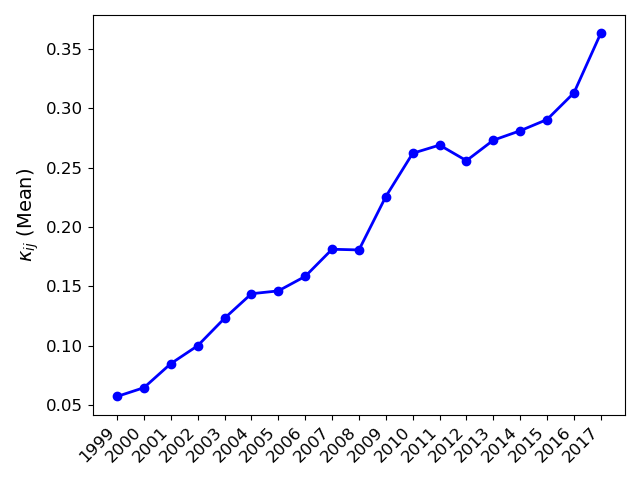
\includegraphics[width=7cm]{figures/kappa}
  \end{center}
\end{frame}

\begin{frame}{Product-Market Rivalry $\bm{\Sigma}$}

  \begin{itemize}
    \item \label{product_identification} \citet{Hoberg2016-jm} estimates product proximity using business descriptions in 10-K
          \medskip{}
    \item \citet{Pellegrino2024-dn} estimates $\alpha$ to align with the cross-price
          elasticity of demand
          \medskip{}
          \[
            \underbrace{\sigma_{ij}}_{\text{substitutability}}=\alpha\times\text{product proximity between }i\text{ and }j\quad\left(i\neq j\right)
          \]\hyperlink{micro_vs_ghl}{\beamerbutton{micro estimates}}
  \end{itemize}

\end{frame}

\begin{frame}{Technological Proximity $\widetilde{\bm{\Omega}}$}
  \begin{itemize}
    \item Technological profile of firm $i$
          \begin{itemize}
            \item The vector of the share of patents held by firm $i$ in each technology class
            \item Baseline: group-level patent classifications ($\approx 4000$), five years window
          \end{itemize}
          \medskip{} \pause
    \item \citet{Jaffe1986-yz} technological proximity measure $\tilde{\omega}_{ij}$:
          \begin{itemize}
            \item Cosine similarity of the technological profiles between firms $i$ and $j$
            \item Impose $\sum_{j\neq i}\tilde{\omega}_{ij} = 1$ for each $i$
          \end{itemize}
  \end{itemize}
\end{frame}

\begin{frame}{Distribution of Knowledge Capital $\bm{z}_t$}
  \begin{table}[htbp]
    \centering
    \begin{tabular}{cl}
      \toprule
      Variables                 & Identification                                                                                                                            \\
      \midrule
      \visible<1->{$\pi_{i,t}$} & \visible<1->{Gross profit (before R\&D cost) $=$ Revenue $-$ Cost of goods sold}                                                          \\[6pt]
      \visible<2->{$\bm{q}_t$}  & \visible<2->{\(\pi_{i,t}=\displaystyle\sum_{j}\kappa_{ij}\,\sigma_{ij}\,q_{i,t}\,q_{j,t}\)}                                               \\[6pt]
      \visible<3->{$\zeta/L$}   & \visible<3->{Matches sample firms' cost share (average markup)}                                                                           \\[6pt]
      \visible<4->{$\bm{z}_t$}  & \visible<4->{\(\displaystyle \bm{z}_{t}=\left\{2\frac{\zeta}{L}\bm{1}_{n\times n}+\bm{\Sigma}+\bm{K}\circ\bm{\Sigma}\right\}\bm{q}_{t}\)} \\
      \bottomrule
    \end{tabular}
  \end{table}
\end{frame}

\begin{frame}{Technology Spillover $\bm{\Omega}=\beta\times$Technological Proximity $\bm{\widetilde{\Omega}}$ \hyperlink{first_stage}{\beamerbutton{First Stage}}}
  \label{regression}
  {\footnotesize
    \[
      \log z_{i,t+1}-\log z_{i,t}
      =\beta\sum_{j\neq i}\tilde{\omega}_{ij,t} \frac{z_{j,t}}{z_{i,t}}
      +\text{Controls}_{i,t}
      +\epsilon_{i,t}
    \] \pause
    \begin{center}
      \setlength{\tabcolsep}{6pt} % Adjust column spacing
      \begin{tabular}{lccc}
        \hline\hline
                         & (1)                                                             & (2)          & (3)          \\
                         & $\log z_{i,t+1}-\log z_{i,t}$
                         & $\log z_{i,t+1}-\log z_{i,t}$
                         & $\log z_{i,t+1}-\log z_{i,t}$                                                                 \\
        \hline
        $\sum_{j\neq i}\tilde{\omega}_{ij,t} \frac{z_{j,t}}{z_{i,t}}$
                         & $\begin{array}{c}\text{0.026}^{**}\\(\text{0.010})\end{array}$
                         & $\begin{array}{c}\text{0.024}^{**}\\(\text{0.010})\end{array}$
                         & $\begin{array}{c}\text{0.073}^{*}\\(\text{0.038})\end{array}$                                 \\
        $\frac{x_{i,t}}{z_{i,t}}$
                         &
                         & $\begin{array}{c}\text{0.514}^{***}\\(\text{0.063})\end{array}$
                         &                                                                                               \\
        \hline
        Firm \& Year FEs & $\checkmark$                                                    & $\checkmark$ & $\checkmark$ \\
        Controls         & $\checkmark$                                                    & $\checkmark$ & $\checkmark$ \\
        IV               &                                                                 &              & $\checkmark$ \\
        Observations     & 14,576                                                          & 14,576       & 14,576       \\
        \hline\hline
      \end{tabular}
    \end{center}
    SEs clustered by years and 4-digit NAICS industries are reported in parentheses. Control variables include $\log z_{i,t}$, firm fixed effects, and year fixed effects.
      {*} $p<\text{0.1}$, {**} $p<\text{0.05}$, {***} $p<\text{0.01}$.}
  \begin{itemize}
    \item IV: User cost of R\&D, driven by federal and state-specific rules variations \citep{Bloom2013-pn}
  \end{itemize}
\end{frame}

\begin{frame}{Identification: Summary}
  \label{identification_summary}
  \begin{itemize}
    \item Publicly available data + Compustat
  \end{itemize}
  \begin{table}[h]
    \centering
    \small % フォントサイズを小さくする
    \begin{tabular}{llll}
      \toprule
      Notation                  & Description                                      & Value & Source                                    \\
      \midrule
      $\bm{\Sigma}$             & Product proximity                                &       & Form 10-K, \citet{Hoberg2016-jm}          \\
      $\bm{\widetilde{\Omega}}$ & Technological proximity                          &       & USPTO, Patent classification              \\
      $\bm{K}$                  & Common ownership weights                         &       & Form 13F, \citet{Backus2021-yt}           \\
      $\alpha$                  & Product proximity $\rightarrow$ Substitutability & 0.120 & \citet{Pellegrino2024-dn}                 \\
      $\beta$                   & Technological proximity $\rightarrow$ Spillovers & 0.024 & Estimated from the law of motion          \\
      $\zeta/L$                 & Labor-augmenting efficiency                      & 0.004 & Compustat, Cost of goods sold             \\
      $\rho$                    & Discount rate                                    & 0.100 &                                           \\
      $\mu$                     & R\&D efficiency                                  & 0.066 & 2.6\% R\&D share (moment match)           \\
      $\delta$                  & Depreciation rate                                & 0.017 & 1.2\% economic growth rate (moment match) \\
      \bottomrule
    \end{tabular}
  \end{table}
  \hyperlink{network_correlation}{\beamerbutton{Network Correlation}}
\end{frame}

\begin{frame}{Model vs. Data: Firm-level Profits, Sales, and R\&D}
  \begin{itemize}
    \item Comparison of firm-level model-generated values ($x$-axis) with observed data ($y$-axis)
  \end{itemize}
  \medskip{}
  \begin{center}
    \begin{figure}
      \centering
      \setcounter{subfigure}{0}
      \subfloat[Log of Profit (Targeted)]{\begin{centering}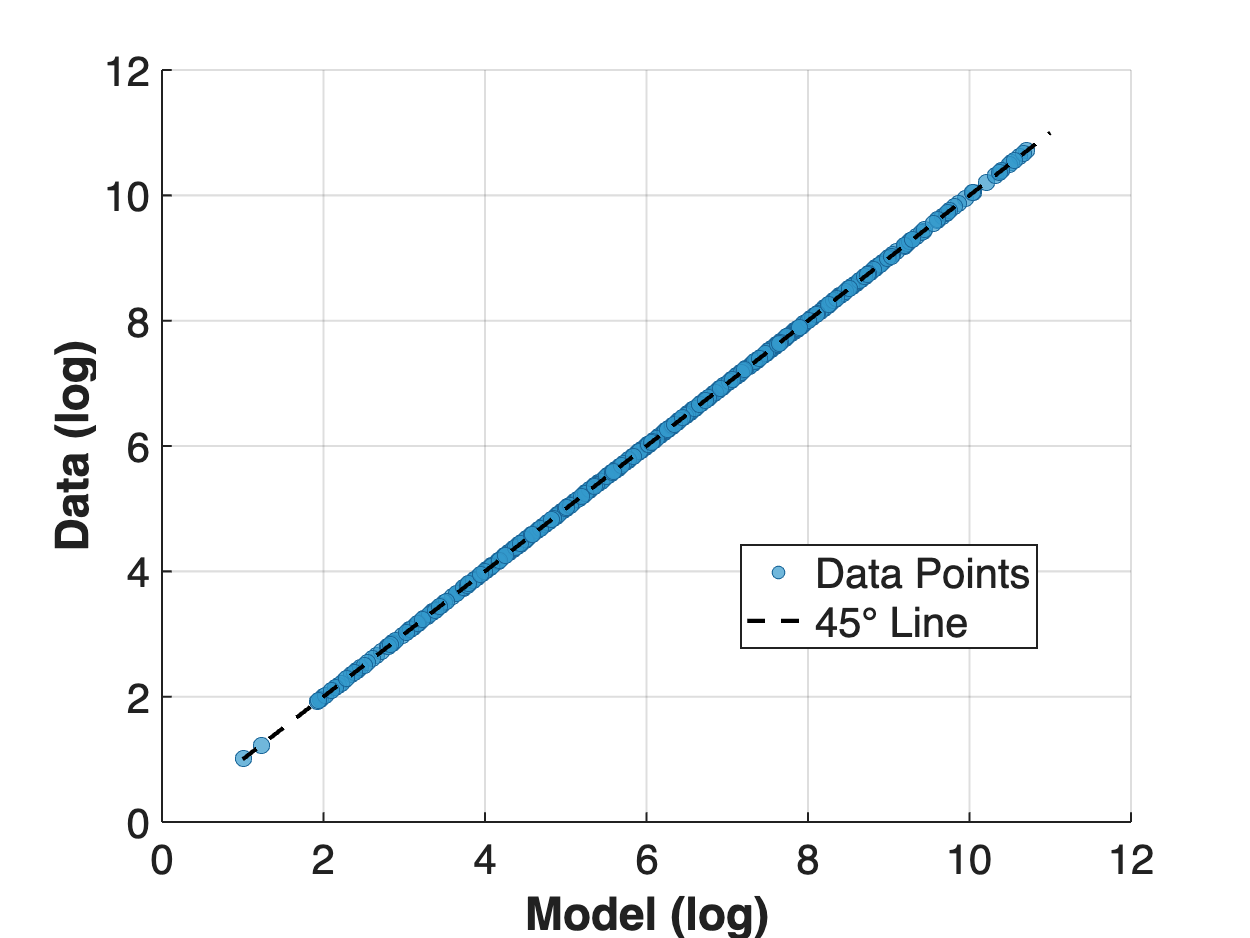
\includegraphics[width=4.5cm]{figures/NO_Profit_vs_data}\par\end{centering}}
      \subfloat[Log of Sales]{\begin{centering}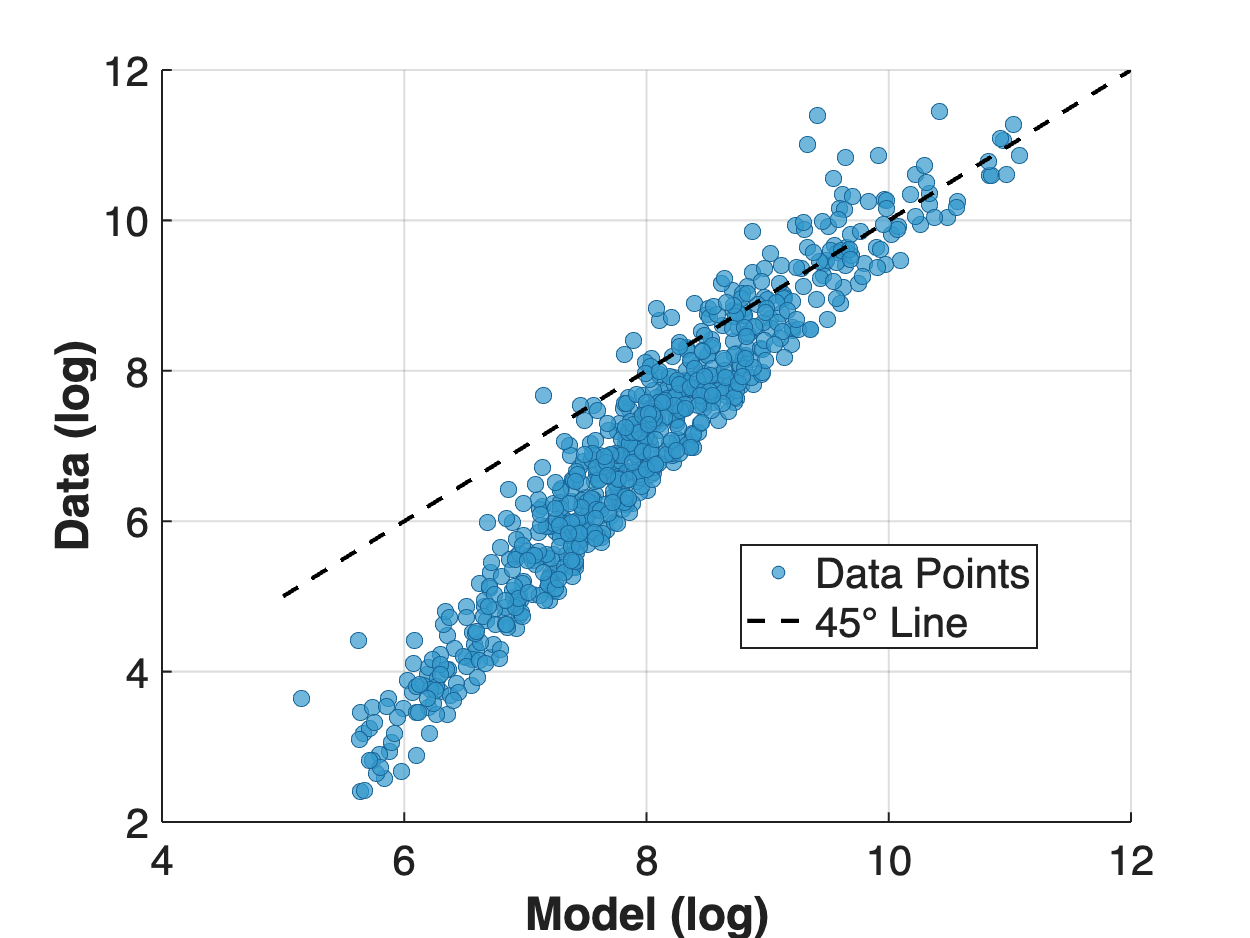
\includegraphics[width=4.5cm]{figures/NO_Sales_vs_data}\par\end{centering}}
      \subfloat[Log of R\&D Expenditure]{\begin{centering}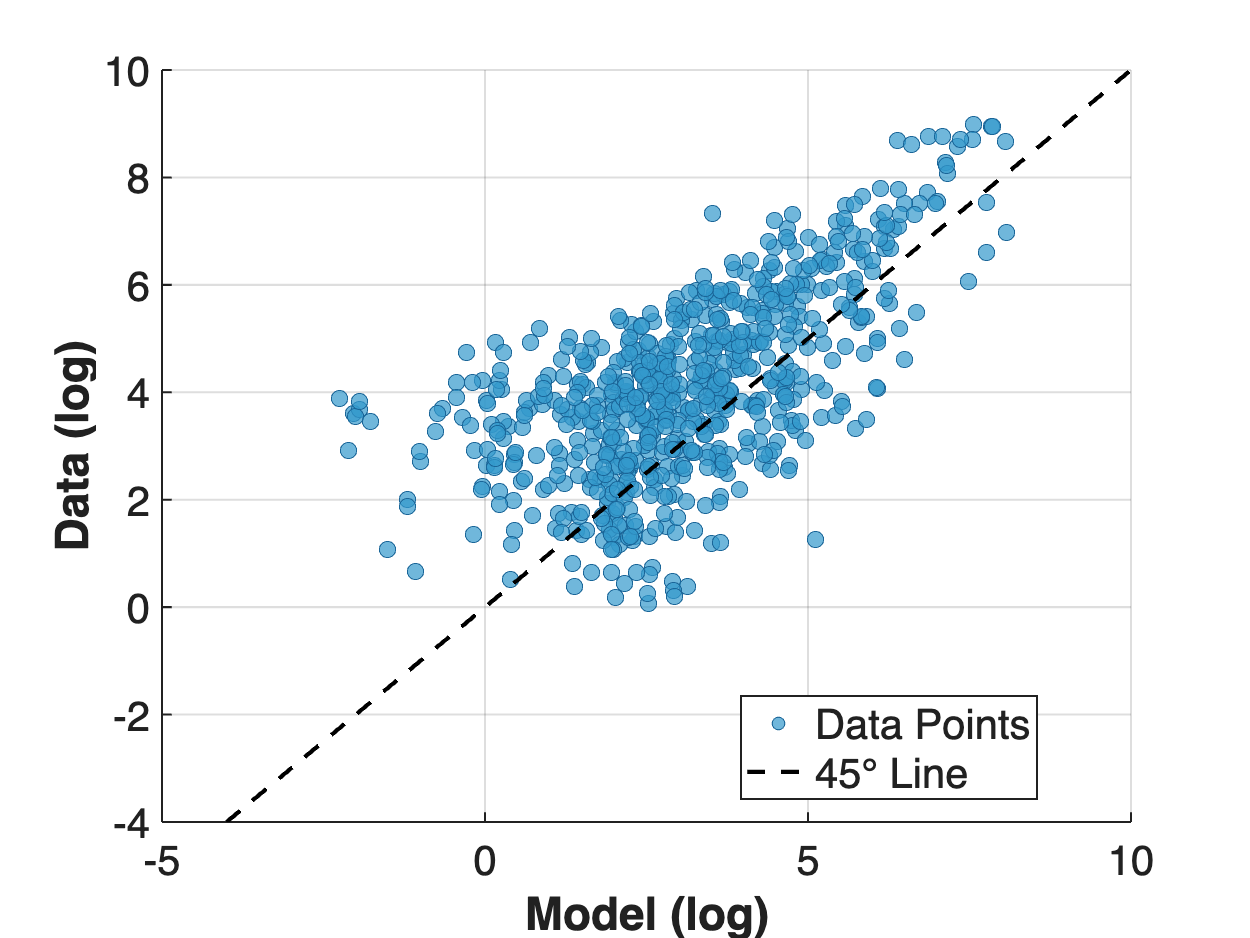
\includegraphics[width=4.5cm]{figures/NO_RnD_vs_data}\par\end{centering}}
    \end{figure}
  \end{center}
\end{frame}

\begin{frame}{Model vs. Data: Firm-level Growth Rates}
  \begin{itemize}
    \item Data: Average growth rate of $z_{i,t}$ between 2010 and 2017
          \medskip{}
    \item Model: Networks and initial knowledge capital in 2010
  \end{itemize}
  \medskip{}
  \begin{center}
    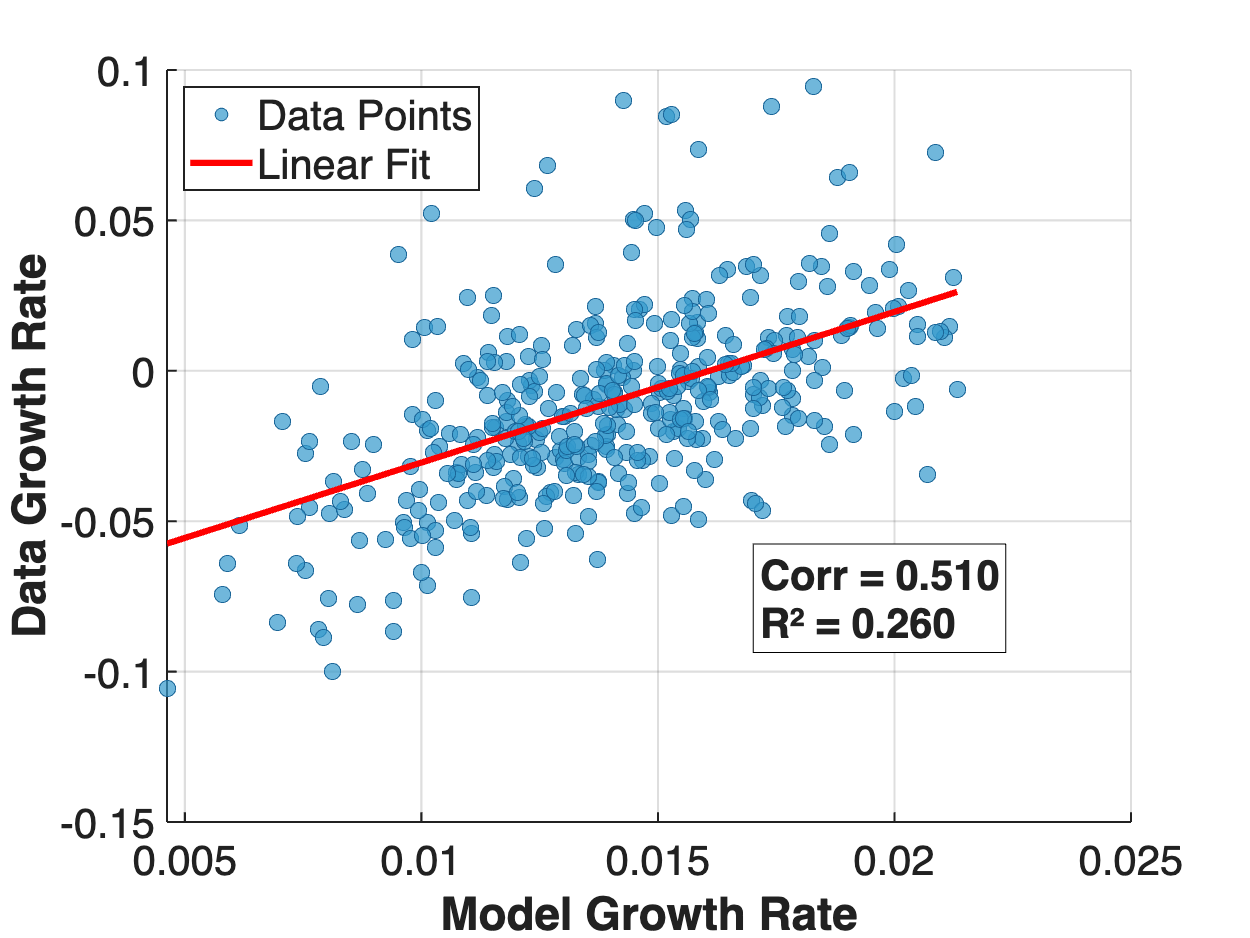
\includegraphics[width=0.5\textwidth]{figures/NO_growth_rate_comparison.png}
  \end{center}
\end{frame}

\begin{frame}{Comparison with \cite{Anton2024-pw}}
  \begin{itemize}
    \item \citet{Anton2024-pw} estimates the effect of interaction b/w common ownership and technology/product proximity on R\&D
  \end{itemize}
  \footnotesize{
    \begin{align*}
      \log\left(1+\text{R\&D}_{it}/A_{it}\right) = & \gamma_1 \log \left(\sum_{j \neq i} \kappa_{ijt} \text{tech proximity}_{ijt} G_{jt}\right) + \gamma_2 \log \left(\sum_{j \neq i} \kappa_{ijt} \text{product proximity}_{ijt} G_{jt}\right) \\  & + \text{Controls}_{it} + \text{Firm FEs}_i + \text{Year FEs}_t + \varepsilon_{ijt}
    \end{align*}
  }
  \begin{table}[h]
    \centering
    \footnotesize
    \begin{tabular}{@{}l l l l l@{}}
      \toprule
      & $\text{R\&D}_{it}$  & $A_{it}$          & $G_{it}$         & Sample period \\
      \midrule
      \cite{Anton2024-pw} & Observed R\&D & Assets            & R\&D stocks        & 1985--2015    \\
      Our model           & Model-generated R\&D& Knowledge capital & Knowledge capital & 1999--2017    \\
      \bottomrule
    \end{tabular}
  \end{table}
  \pause
  \begin{table}[h]
    \centering
    \footnotesize
    \begin{tabular}{@{}l cc@{}}
      \toprule
                                                                                             & \cite{Anton2024-pw}           & Our model \\
      \midrule
      $\log \left(\sum_{j \neq i} \kappa_{ijt} \text{tech proximity}_{ijt} G_{jt}\right)$    & \shortstack{$0.00513^{**}$ \\ $(0.00226)$} & \shortstack{$0.00194^{***}$ \\ $(0.000272)$} \\
      $\log \left(\sum_{j \neq i} \kappa_{ijt} \text{product proximity}_{ijt} G_{jt}\right)$ & \shortstack{$-0.00457^{**}$ \\ $(0.00222)$} & \shortstack{$-0.00547^{***}$ \\ $(0.000693)$} \\
      \bottomrule
    \end{tabular}
  \end{table}
\end{frame}

\section{Exercise}

\begin{frame}{Counterfactual Ownership Structures}
  \begin{table}[h]
    \centering
    \renewcommand{\arraystretch}{1.5} % 行間を広げる
    \begin{tabular}{ll}
      \toprule
      Ownership Structure       & Description                                                                                                                                                                           \\
      \midrule
      \visible<1->{Baseline}    & \visible<1->{Observed common ownership structure in 2017}                                                                                                                             \\
      \visible<2->{Dispersed}   & \visible<2->{$\bm{K}^D=\bm{I}$}                                                                                                                                                       \\
      \visible<3->{Mean$=$1999} & \visible<3->{\(\kappa_{ij,2017}^{M1999}=\text{const}\times\kappa_{ij,2017}\) and \(\bm{E}\left[\kappa_{ij,2017}^{M1999}\right]=\bm{E}\left[\kappa_{ij,1999}\right]\) for \(j\neq i\)} \\
      \visible<4->{Uniform}     & \visible<4->{\(\kappa_{ij,2017}^U=\bm{E}\left[\kappa_{ij, 2017}\right]\) for \(j\neq i\)}                                                                                             \\
      \visible<5->{Monopoly}    & \visible<5->{$\bm{K}^M=\bm{1}_{n\times n}$}                                                                                                                                           \\
      \bottomrule
    \end{tabular}
    \renewcommand{\arraystretch}{1.0}
  \end{table}
\end{frame}

\begin{frame}{Total R\&D Expenditure}

  \begin{itemize}
    \item For the moment, assume that ownership structure only affects R\&D decisions
          \begin{itemize}
            \item Product-market competition: firms maximize gross profits (dispersed ownership)
          \end{itemize}
  \end{itemize}
  \medskip{}\pause
  \begin{center}
    \setlength{\tabcolsep}{3pt}
    \begin{tabular}{@{} c *{5}{c} @{}}
      \toprule
      \multirow{2}{*}{\shortstack[t]{Total R\&D in 2017                                                                      \\ (Optimal R\&D: 100)}}
       & \multicolumn{5}{c}{Ownership Structure}                                                                             \\
      \cmidrule(lr){2-6}
       & Dispersed
       & Mean$=$1999
       & Uniform
       & Baseline
       & Monopoly                                                                                                            \\
      \midrule
      Baseline
       & 40.48                                   & \textcolor{uclaBlue}{38.68} & 31.56 & \textcolor{uclaBlue}{28.26} & 21.39 \\
      \midrule
      \shortstack[t]{Only Business Steal                                                                                     \\ $\bm{\Omega}=[0]$}
       & \visible<3->{52.04}
       & \visible<3->{49.73}
       & \visible<3->{41.51}
       & \visible<3->{36.40}
       & \visible<3->{30.69}                                                                                                 \\
      \midrule
      \shortstack[t]{Only Tech Spill                                                                                         \\ $\bm{\Sigma}=\bm{I},\,\zeta/L=0$}
       & \visible<4->{13.61}
       & \visible<4->{14.25}
       & \visible<4->{18.33}
       & \visible<4->{19.33}
       & \visible<4->{27.77}                                                                                                 \\
      \bottomrule
    \end{tabular}
  \end{center}
  \medskip{}
  \begin{itemize}
    \item Internalization of business-stealing $>$ internalization of technology spillovers
  \end{itemize}
\end{frame}

\begin{frame}{Total R\&D, Growth Rate, Social Welfare, Firm Value Share}
  \label{results}
  \centering
  \setlength{\tabcolsep}{3pt}
  \begin{tabular}{@{} c *{5}{c} @{}}
    \toprule
    \multirow{2}{*}{\shortstack[t]{}} & \multicolumn{5}{c}{Ownership Structure}                                                                                                                                     \\
    \cmidrule(lr){2-6}
                                      & Dispersed
                                      & Mean$=$1999
                                      & Uniform
                                      & Baseline
                                      & Monopoly                                                                                                                                                                    \\
    \midrule
    \shortstack[l]{Total R\&D (Optimal R\&D: 100)}
                                      & 40.48                                   & 38.68                                     & 31.56               & 28.26                                     & 21.39               \\
    \midrule
    \shortstack[l]{Economic Growth Rate (\%)}
                                      & \visible<2->{1.32}                      & \visible<2->{\textcolor{uclaBlue}{1.31}}  & \visible<2->{1.24}  & \visible<2->{\textcolor{uclaBlue}{1.20}}  & \visible<2->{1.11}  \\
    \midrule
    \shortstack[l]{CE Welfare (Optimal R\&D: 100)}
                                      & \visible<3->{94.91}                     & \visible<3->{\textcolor{uclaBlue}{94.86}} & \visible<3->{94.52} & \visible<3->{\textcolor{uclaBlue}{94.35}} & \visible<3->{93.47} \\
    \midrule
    \shortstack[l]{Firm Value Share (\%)}
                                      & \visible<4->{26.63}                     & \visible<4->{26.72}                       & \visible<4->{27.20} & \visible<4->{27.24}                       & \visible<4->{27.82} \\
    \bottomrule
  \end{tabular}
  \medskip{}
  \begin{itemize}
    \item The rise of common ownership from 1999 to 2017 $\Longrightarrow$ \visible<2->{$g$ $\downarrow$ by 0.11 p.p.,} \visible<3->{CE welfare $\downarrow$ by 0.54\%}
          \medskip{}
    \item The results are qualitatively the same under different corporate governance assumptions \hyperlink{corporate_governance}{\beamerbutton{Corporate Governance Assumptions}}
  \end{itemize}
\end{frame}

\begin{frame}{When Common Ownership Affects Both R\&D and Production}
  \begin{center}
    \setlength{\tabcolsep}{3pt}
    \begin{tabular}{@{}lccc@{}}
      \toprule
      \multicolumn{1}{l}{Production ownership structure} & Dispersed & Dispersed                   & Common                      \\
      \multicolumn{1}{l}{R\&D ownership structure}       & Dispersed & Common                      & Common                      \\
      \midrule
      \shortstack[l]{Total Output (Dispersed: 100)}
                                                         & 100.00    & 100.00                      & 97.26                       \\
      \shortstack[l]{Total R\&D (Dispersed: 100)}
                                                         & 100.00    & \textcolor{uclaBlue}{69.81} & \textcolor{uclaBlue}{86.36} \\
      \shortstack[l]{Economic Growth Rate (\%)}
                                                         & 1.323     & 1.200                       & 1.288                       \\
      \shortstack[l]{CE Welfare (Dispersed: 100)}
                                                         & 100.00    & 99.41                       & 97.28                       \\
      \shortstack[l]{Firm Value Share (\%)}
                                                         & 26.63     & 27.24                       & 34.10                       \\
      \bottomrule
    \end{tabular}
  \end{center}
  \medskip{}
  \begin{itemize}
    \item Less product market competition $\Longrightarrow$ Private return on R\&D $\uparrow$
  \end{itemize}
\end{frame}

\begin{frame}{Optimal Uniform R\&D Subsidy}
  \begin{center}
    \begin{figure}
      \centering
      \setcounter{subfigure}{0}
      \subfloat[Economic Growth]{\begin{centering}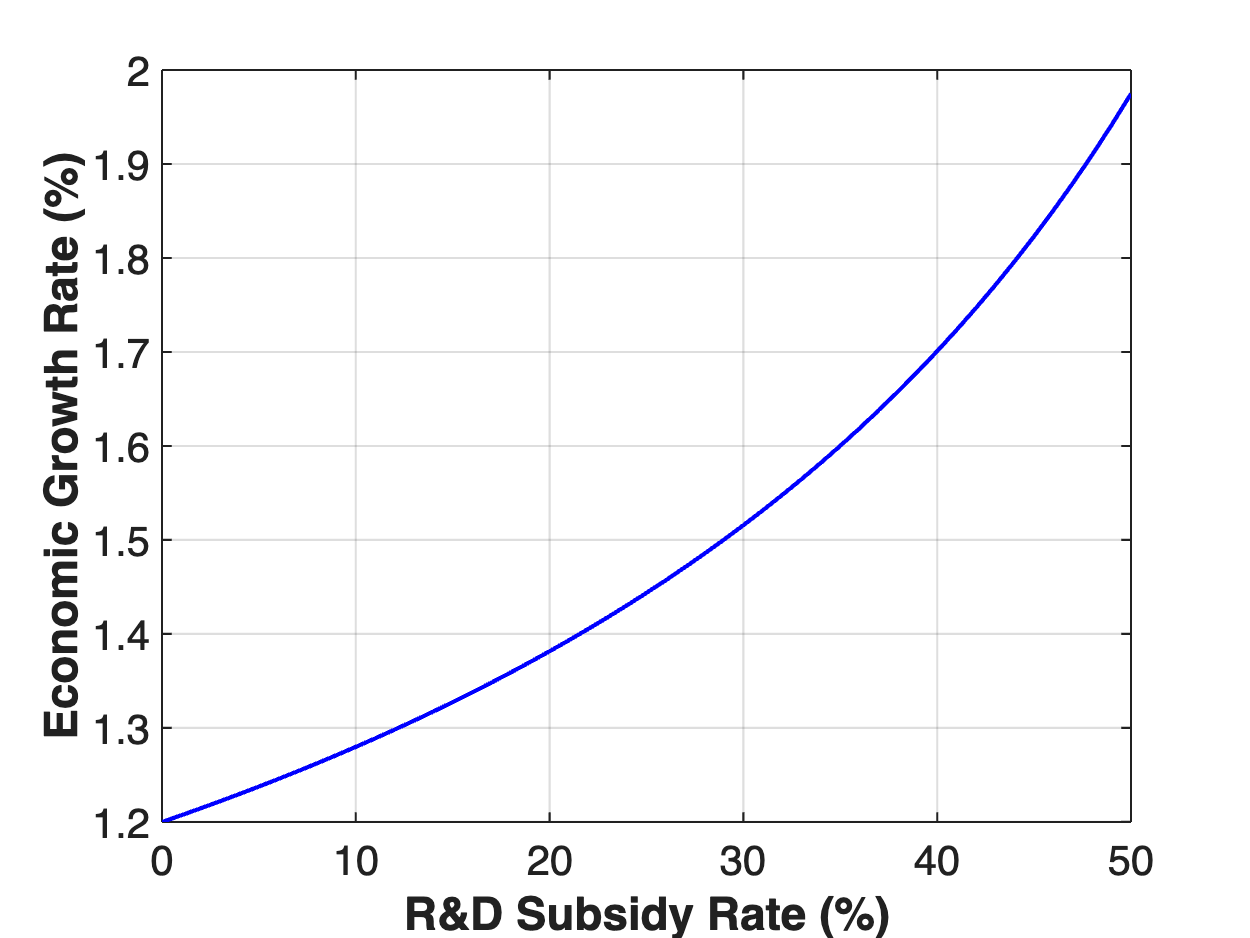
\includegraphics[width=6cm]{figures/subsidy_growth_rate}\par\end{centering}}
      \subfloat[Social Welfare]{\begin{centering}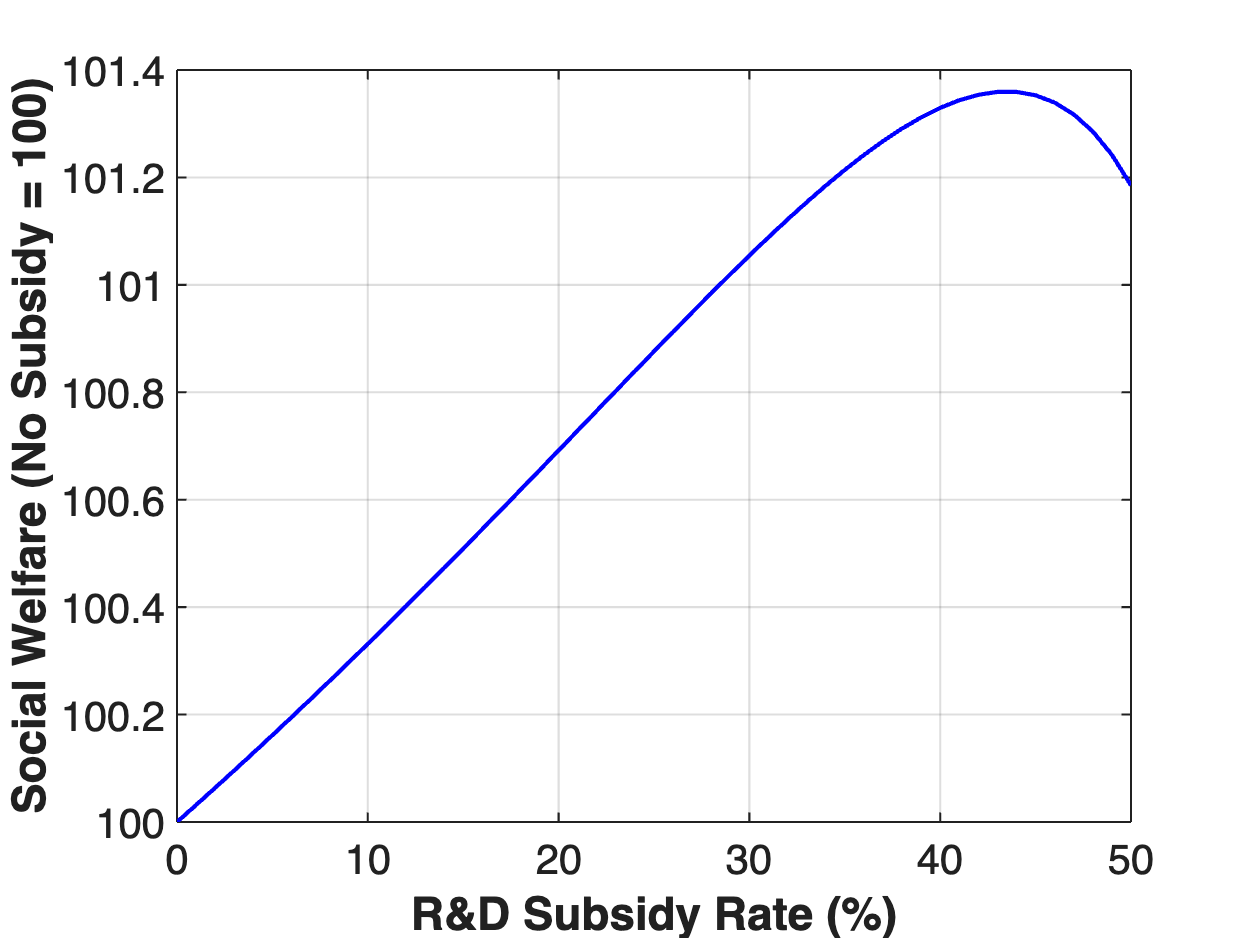
\includegraphics[width=6cm]{figures/subsidy_social_welfare}\par\end{centering}}
    \end{figure}
  \end{center}
  \begin{itemize}
    \item Optimal rate is $s=43\%$, which increases $g$ by 0.57 pp and CE welfare by 1.36\%
    \item c.f. Welfare gains from optimal R\&D allocation: 6.0\%
  \end{itemize}
\end{frame}

\begin{frame}{Which Firms' R\&D Should be Subsidized?}

  \begin{center}
    \setlength{\tabcolsep}{6pt}
    \begin{tabular}{lcc}
      \hline\hline
                                      & Private R\&D $x$                                                   & Social / Private value of R\&D                                                              \\
      \hline
      Initial knowledge capital $z$   & $\begin{array}{c}\text{0.122}^{***}\\(\text{0.000848})\end{array}$ & $\begin{array}{c}\text{-0.000212}\\(\text{0.000158})\end{array}$                            \\
      Product market centrality       & $\begin{array}{c}\text{-16.4}^{***}\\(\text{0.286})\end{array}$    & $\begin{array}{c}\textcolor{uclaBlue}{\text{-1.06}^{***}}\\(\text{0.0532})\end{array}$ \\
      Technology spillover centrality & $\begin{array}{c}\text{5.45}^{***}\\(\text{0.423})\end{array}$     & $\begin{array}{c}\textcolor{uclaBlue}{\text{1.48}^{***}}\\(\text{0.0788})\end{array}$ \\
      Ownership structure centrality  & $\begin{array}{c}\text{-7.16}^{***}\\(\text{0.239})\end{array}$    & $\begin{array}{c}\textcolor{uclaBlue}{\text{0.580}^{***}}\\(\text{0.0446})\end{array}$ \\
      Intercept                       & $\begin{array}{c}\text{-22.4}^{***}\\(\text{0.255})\end{array}$    & $\begin{array}{c}\text{0.900}^{***}\\(\text{0.0475})\end{array}$                            \\
      \hline
      Observations                    & \multicolumn{1}{c}{740}                                            & \multicolumn{1}{c}{740}                                                                     \\
      $R^2$                           & \multicolumn{1}{c}{0.976}                                          & \multicolumn{1}{c}{0.555}                                                                   \\
      \hline\hline
    \end{tabular}
  \end{center}
\end{frame}


\begin{frame}{Alternative Corporate Governance Models}
  \label{corporate_governance}
  \begin{enumerate}
    \item Baseline proportional influence: $\kappa_{ij}=\frac{\sum_{o} s_{io}s_{jo}}{\sum_{o}s_{io}^2}$ \medskip{}
    \item Super-proportional influence: $\kappa^{SP}_{ij}=\frac{\sum_{o}\gamma_{io}s_{io}s_{jo}}{\sum_{o}\gamma_{io}s_{io}^2}$ where $\gamma_{io}=\sqrt{s_{io}}$
          \medskip{}\pause
    \item Blockholder influence: $\kappa^{BH}_{ij}=\frac{\sum_{o}b_{io}s_{io}s_{jo}}{\sum_{o}s_{io}^2}\quad(i\neq j),$ where $b_{io}=1$ if $s_{io}>5\%$
          \medskip{}\pause
    \item Structural estimation in the airline industry by \citet{Azar2021-mb}: $\kappa^{AR}_{ij} = \tau_{i}\kappa_{ij}\quad(i\neq j)$ 
    \begin{enumerate}
      \item Uniform: $\tau = 0.29$
      \item Firm-specific: $\tau_{i}=\frac{\exp\left[\theta_{0}+\log\left(\text{Investor HHI}_{i}\right)\right]}{1+\exp\left[\theta_{0}+\log\left(\text{Investor HHI}_{i}\right)\right]}$ where $\theta_{0}=2.68$
    \end{enumerate}
  \end{enumerate}
\end{frame}

\begin{frame}{Alternative Corporate Governance Models}

  {\footnotesize
  \begin{center}
  \begin{tabular}{@{}lcccccc@{}}
    \toprule
     & \multicolumn{6}{c}{Ownership Structure}                                         \\
    \midrule
     & \shortstack{Dispersed                                                                   \\ Ownership}
     & \shortstack{Baseline:                                                                   \\ Proportional \\ Influence}
     & \shortstack{Super                                                                       \\ Proportional \\ Influence}
     & \shortstack{Blockholder                                                                 \\ Influence}
     &  \shortstack{AR  \\ Uniform}
     & \shortstack{AR \\ Firm-Specific} \\
    \midrule
    \shortstack[l]{Total R\&D Expenditure}
     & 100.00                                          & \textcolor{uclaBlue}{69.81} &\textcolor{uclaBlue}{68.97} & \textcolor{uclaBlue}{77.45} & \textcolor{uclaBlue}{90.32} & \textcolor{uclaBlue}{90.41} \\
    \shortstack[l]{Growth Rate (\%) }
     & 1.323                                           & 1.200 & 1.194 & 1.234 & 1.287 & 1.289 \\
    \shortstack[l]{CE Welfare}
     & 100.00                                          & 99.41 & 99.37 & 99.59 & 99.86 & 99.86 \\
    \shortstack[l]{Firm Value Share (\%) }
     & 26.63                                           & 27.24 & 27.24 & 27.09 & 26.82 & 26.84 \\
    \bottomrule
  \end{tabular}
  \end{center}
  }
  \medskip{}
  \begin{itemize}
    \item Internalization of business-stealing $>$ internalization of technology spillovers
  \end{itemize}
\end{frame}

\section{Conclusion}
\label{conclusion}
\begin{frame}{Conclusion}
  \begin{itemize}
    \item Quantitative Schumpeterian growth model with ownership structure
          \begin{itemize}
            \item Utilizes micro data and computational capabilities
          \end{itemize}
          \medskip{}
    \item Common ownership in the U.S.:
          \begin{enumerate}
            \item Internalization of business-stealing effect $\Longrightarrow$ $g$ $\downarrow\downarrow$
            \item Internalization of technology spillover effect $\Longrightarrow$ $g$ $\uparrow$
          \end{enumerate}
          \medskip{}
    \item Potential applications:
          \begin{itemize}
            \item M\&A
            \item Conglomerate (e.g. Korea)
            \item Cross-shareholdings (e.g. Japan, Germany, AI companies \hyperlink{ai}{\beamerbutton{AI}})
            \item FDI and international technology diffusion
            \item Technology licensing
          \end{itemize}
  \end{itemize}
\end{frame}

\appendix
\section{Appendix}

\begin{frame}{Share of Top 5 Shareholders in Largest Market Cap Firms \hyperlink{intro}{\beamerbutton{Back}}}
  \label{share}
  % --- 1行目 ---
  \begin{minipage}[t]{0.3\textwidth} % 1番目: Microsoft
    \centering
    \footnotesize % <--- \scriptsize から変更
    \begin{tabular}{lr}
      \toprule
      Microsoft            &        \\
      \midrule
      \alert{Vanguard}     & 9.20\% \\
      \alert{Blackrock}    & 7.75\% \\
      Steven Ballmer       & 4.48\% \\
      \alert{State Street} & 3.97\% \\
      \alert{Fidelity}     & 2.66\% \\
      \bottomrule
    \end{tabular}
  \end{minipage}
  \hfill % スペース
  \begin{minipage}[t]{0.3\textwidth} % 2番目: Nvidia
    \centering
    \footnotesize % <--- \scriptsize から変更
    \begin{tabular}{lr}
      \toprule
      Nvidia               &        \\
      \midrule
      \alert{Vanguard}     & 8.93\% \\
      \alert{BlackRock}    & 7.74\% \\
      \alert{Fidelity}     & 4.12\% \\
      \alert{State Street} & 3.97\% \\
      Jensen Huang         & 3.80\% \\
      \bottomrule
    \end{tabular}
  \end{minipage}
  \hfill % スペース
  \begin{minipage}[t]{0.3\textwidth} % 3番目: Apple
    \centering
    \footnotesize % <--- \scriptsize から変更
    \begin{tabular}{lr}
      \toprule
      Apple                &        \\
      \midrule
      \alert{Vanguard}     & 9.29\% \\
      \alert{Blackrock}    & 7.48\% \\
      \alert{State Street} & 3.96\% \\
      \alert{Fidelity}     & 2.27\% \\
      Geode Capital        & 2.26\% \\
      \bottomrule
    \end{tabular}
  \end{minipage}

  \vspace{0.5cm} % 行間の垂直スペース

  % --- 2行目 ---
  \begin{minipage}[t]{0.3\textwidth} % 4番目: Google
    \centering
    \footnotesize % <--- \scriptsize から変更
    \begin{tabular}{lr}
      \toprule
      Google               &        \\
      \midrule
      \alert{Vanguard}     & 7.36\% \\
      \alert{Blackrock}    & 6.47\% \\
      \alert{State Street} & 3.39\% \\
      \alert{Fidelity}     & 3.01\% \\
      Sergey Brin          & 2.99\% \\
      \bottomrule
    \end{tabular}
  \end{minipage}
  \hfill % スペース
  \begin{minipage}[t]{0.3\textwidth} % 5番目: Amazon
    \centering
    \footnotesize % <--- \scriptsize から変更
    \begin{tabular}{lr}
      \toprule
      Amazon               &        \\
      \midrule
      Jeffrey Bezos        & 8.58\% \\
      \alert{Vanguard}     & 7.77\% \\
      \alert{Blackrock}    & 6.50\% \\
      \alert{State Street} & 3.44\% \\
      \alert{Fidelity}     & 3.10\% \\
      \bottomrule
    \end{tabular}
  \end{minipage}
  \hfill % スペース
  \begin{minipage}[t]{0.3\textwidth} % 6番目: Meta
    \centering
    \footnotesize % <--- \scriptsize から変更
    \begin{tabular}{lr}
      \toprule
      Meta                 &        \\
      \midrule
      \alert{Vanguard}     & 7.55\% \\
      \alert{Blackrock}    & 6.50\% \\
      \alert{Fidelity}     & 5.38\% \\
      Accel IX LP          & 3.88\% \\
      \alert{State Street} & 3.40\% \\
      \bottomrule
    \end{tabular}
  \end{minipage}
\end{frame}

\begin{frame}{Merger Guidelines \hyperlink{intro}{\beamerbutton{Back}}}
  \label{guidelines}
  \begin{quote}
    ``For example, \alert{the partial owner may decide not to develop a new product feature} to win market share from the firm in which it has acquired an interest, because doing so will reduce the value of its investment in its rival.''
  \end{quote}
  \medskip{}
  2023 Merger Guidelines by the U.S. Department of Justice and the Federal Trade Commission
\end{frame}

\begin{frame}{Cross Shareholdings among AI Companies \hyperlink{conclusion}{\beamerbutton{Back}}}
  \label{ai}
  \begin{figure}
    \centering
    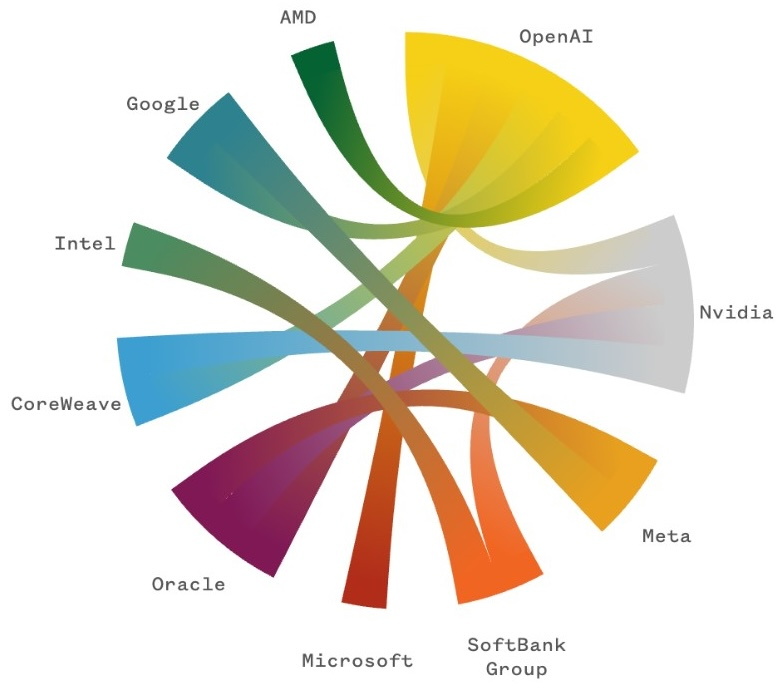
\includegraphics[width=0.45\textwidth]{figures/AI_circular.jpeg}
  \end{figure}
  {\footnotesize Source: \href{https://longbridge.com/en/news/260114348}{Wallstreetcn.com}}
\end{frame}

\begin{frame}{Technology \& Product Proximity: Example}
  % --- Use columns environment for side-by-side content ---
  \begin{columns}[T] % [T] aligns content at the top
    % --- Left Column ---
    \begin{column}{0.45\textwidth} % Adjust width as needed
      \centering % Center the content within the column
      \begin{tabular}{lr}
        \toprule
        Tesla vs. Ford       &      \\
        \midrule
        Technology Proximity & 0.11 \\
        Product Proximity    & 0.15 \\ % Note the % sign
        \bottomrule
      \end{tabular}
    \end{column}
    % --- Right Column ---
    \begin{column}{0.45\textwidth} % Adjust width as needed
      \centering % Center the content within the column
      \begin{tabular}{lr}
        \toprule
        Apple vs. Intel      &      \\
        \midrule
        Technology Proximity & 0.57 \\
        Product Proximity    & 0.00 \\ % Note: No % sign here
        \bottomrule
      \end{tabular}
    \end{column}
  \end{columns}
\end{frame}

\begin{frame}{Empirical Literature: Common Ownership $\Longrightarrow$ R\&D}
  \begin{itemize}
    \item \cite{Anton2024-pw}:
          \begin{itemize}
            \item Dependent variables: R\&D, citation-weighted patents, market value of patents
                  \begin{itemize}
                    \item[+] Interaction term between common ownership and technology proximity
                    \item[--] Interaction term between common ownership and product proximity
                  \end{itemize}
          \end{itemize} \medskip{}
    \item \cite{Kini2024-kd}: DiD that exploits mergers between financial institutions
          \begin{itemize}
            \item Dependent variables: Investments, new product development
                  \begin{itemize}
                    \item[+] Post (merger) $\times$ treatment (common owner) $\times$ technology proximity
                  \end{itemize}
          \end{itemize}
  \end{itemize}
\end{frame}

\begin{frame}{R\&D Externalities}
  \label{rd_externalities} % <--- この行を追加
  \begin{enumerate}
    \item Business-stealing effect
          \begin{itemize}
            \item Innovators steal the business (profits) of other firms
          \end{itemize}
          \medskip{}
    \item Technology spillover effect
          \begin{itemize}
            \item Innovation improves the productivity of other firms
          \end{itemize}
          \medskip{}
    \item Appropriability effect (market power)
          \begin{itemize}
            \item Innovators cannot appropriate the entire consumer surplus
          \end{itemize}
  \end{enumerate}
\end{frame}

\begin{frame}{Generalized Hedonic-Linear Demand \citep{Pellegrino2024-dn}}
  \label{ghl}
  \begin{itemize}
    \item $i\in\left\{ 1,2,...,n\right\} $: firms / products
    \item 1 unit of product $i$ provides
          \begin{itemize}
            \item 1 unit of idiosyncratic characteristic $k\in\left\{ 1,2,...,n\right\} $
            \item ${\color{uclaBlue}\psi{}_{k,i}}$ unit of shared characteristic $k\in\left\{ n+1,n+2,...,n+n_{k}\right\} $ where $\sum_{k}{\color{uclaBlue}\psi_{k,i}^{2}}=1$
          \end{itemize}
    \item Aggregate each characteristic:
          \[
            y_{k,t}=\begin{cases}
              q_{k,t}                                       & k=1,2,...,n           \\
              \sum_{i}{\color{uclaBlue}\psi{}_{k,i}}q_{i,t} & k=n+1,n+2,...,n+n_{k}
            \end{cases}
          \]
    \item Linear-quadratic aggregator over characteristics:
          \[
            Y_{t}=\left(1-\alpha\right)\sum_{k=1}^{n}\left(\underbrace{\hat{b}_{k,t}y_{k,t}-\frac{1}{2}y_{k,t}^{2}}_{\text{idiosyncratic characteristic}}\right)+\alpha\sum_{k=n+1}^{n+n_{k}}\left(\underbrace{\hat{b}_{k,t}y_{k,t}-\frac{1}{2}y_{k,t}^{2}}_{\text{shared characteristic}}\right)
          \]
  \end{itemize}
\end{frame}

\begin{frame}{Generalized Hedonic-Linear Demand \citep{Pellegrino2024-dn}}
  \begin{itemize}
    \item Quality:
          \[
            b_{i}=\left(1-\alpha\right)\hat{b}_{i}+\alpha\sum_{k=n+1}^{n+n_{k}}\psi_{k}\hat{b}_{k}
          \]
    \item Inverse demand:
          \[
            \frac{\bm{p}}{P}=\bm{b}-\bm{\Sigma}\bm{q}
          \]
    \item Inverse cross-price elasticity of demand:
          \[
            \frac{\partial\log p_{i}}{\partial\log q_{j}}=-\frac{q_{j}}{p_{i}}\cdot\sigma_{ij}
          \]
    \item Cross-price elasticity of demand:
          \[
            \frac{\partial\log q_{i}}{\partial\log p_{j}}=-\frac{p_{j}}{q_{i}}(\bm{\Sigma}^{-1})_{ij}
          \]
  \end{itemize}
\end{frame}

\begin{frame}{Static Profits}
  \label{Q}
  \begin{itemize}
    \item Firms choose labor productivity and product quality: $\zeta a_{i,t}=\sqrt{\zeta w_{t}}$, $b_{i,t}=z_{i,t}-\sqrt{\zeta w_{t}}$
    \item Labor market clearing: $L=\sum_{i}\frac{q_{i,t}}{a_{i,t}}$ $\Longrightarrow$$\sqrt{\zeta w_{t}}=\frac{\zeta}{L}\sum_{i}q_{i,t}$
    \item $\bm{q}_{t}=\bm{N}\bm{z}_{t}$ where $\bm{N}\equiv\left\{ 2\frac{\zeta}{L}\bm{J}+\bm{\Sigma}+\bm{K}\circ\bm{\Sigma}\right\} ^{-1}$
    \item $\bm{N}_{i}$: the $i$th row of $\bm{N}$
    \item Ownership weighted profit:
          {\small
          \[
            \sum_{j}\kappa_{ij}\frac{\pi_{j,t}}{P_{t}}=\sum_{j}\kappa_{ij}\sum_{h}\kappa_{jh}\sigma_{jh}q_{j,t}q_{h,t}=\bm{z}_{t}^{T}\bm{Q}^{i}\bm{z}_{t}
          \]}
          where
            {\small
              \[
                \bm{Q}^{i}=\frac{1}{2}\sum_{j}\kappa_{ij}\sum_{h}\kappa_{jh}\sigma_{jh}\left(N_{j}^{T}N_{h}+N_{h}^{T}N_{j}\right)
              \]}
          \hyperlink{dynamic_game}{\beamerbutton{Back}}
  \end{itemize}
\end{frame}

\begin{frame}{Riccati Equations}
  \label{riccati}
  \begin{itemize}
    \item $V^{i}\left(\bm{z}\right)=\bm{z}^{T}\bm{X}^{i}\bm{z}$ where $\bm{X}^{i}$ is the solution of the stacked Riccati equation
            {\small
              \[
                0=\bm{Q}^{i}-\mu^{2}\sum_{j}\kappa_{ij}\bm{X}_{j}^{j}\left(\bm{X}_{j}^{j}\right)^{T}+\left(\bm{\Phi}-\frac{1}{2}\left(\rho-\gamma^{2}\right)\bm{I}\right)^{T}\bm{X}^{i}+\bm{X}^{i}\left(\bm{\Phi}-\frac{1}{2}\left(\rho-\gamma^{2}\right)\bm{I}\right)
              \]}
          \begin{itemize}
            \item $\bm{X}_{i}^{i}\equiv$ the $i$th column of $\bm{X}^{i}$
            \item $\bm{\Phi}\equiv\bm{\Omega}+\mu^{2}\left[\begin{array}{ccc}\bm{X}_{1}^{1} & \cdots & \bm{X}_{n}^{n}\end{array}\right]^{T}$
          \end{itemize}
          \medskip{}
    \item Algorithm: Given $\left[\begin{array}{ccc}\bm{X}_{\tau}^{1} & \cdots & \bm{X}_{\tau}^{n}\end{array}\right]$, update $\left[\begin{array}{ccc}\bm{X}_{\tau-\Delta}^{1} & \cdots & \bm{X}_{\tau-\Delta}^{n}\end{array}\right]$ by
            {\small
              \[
                -\frac{\bm{X}_{\tau}^{i}-\bm{X}_{\tau-\Delta}^{i}}{\Delta}=\bm{Q}^{i}-\mu^{2}\sum_{j}\kappa_{ij}\bm{X}_{j,\tau}^{j}\left(\bm{X}_{j,\tau}^{j}\right)^{T}+\left(\bm{\Phi}_{\tau}-\frac{1}{2}\left(\rho-\gamma^{2}\right)\bm{I}\right)^{T}\bm{X}_{\tau}^{i}+\bm{X}_{\tau}^{i}\left(\bm{\Phi}_{\tau}-\frac{1}{2}\left(\rho-\gamma^{2}\right)\bm{I}\right)
              \]}
  \end{itemize}
  \hyperlink{hjb}{\beamerbutton{Back}}
\end{frame}


\begin{frame}{Summary of Equilibrium}
  \label{summary}
  \begin{center}
    \begin{tabular}{ll}
      Description                     & Expression\tabularnewline
      \hline
      Production strategy             & $\bm{q}_{t}=\bm{N}\bm{z}_{t}$\tabularnewline
      R\&D strategy                   & $\bm{x}_{t}=\mu\tilde{\bm{X}}\bm{z}_{t}$\tabularnewline
      Law of motion                   & $d\bm{z}_{t}=\left(\bm{\Omega}\bm{z}_{t}+\mu\bm{x}_{t}\right)dt+\gamma\bm{z}_{t}dW_{t}$\tabularnewline
      Profit of final producers       & $\Pi_{t}^{F}/P_{t}=\bm{q}_{t}^{T}\left(\frac{1}{2}\bm{\Sigma}\right)\bm{q}_{t}$\tabularnewline
      Total operating profit of firms & $\Pi_{t}/P_{t}=\bm{q}_{t}^{T}\left(\frac{1}{2}\bm{\Sigma}\circ\left(\bm{K}+\bm{K}^{T}\right)\right)\bm{q}_{t}$\tabularnewline
      Labor income                    & $w_{t}L/P_{t}=\bm{q}_{t}^{T}\left(\frac{\zeta}{L}\bm{J}\right)\bm{q}_{t}$\tabularnewline
      Output                          & $Y_{t}=\bm{q}_{t}^{T}\left(\frac{\zeta}{L}\bm{J}+\frac{1}{2}\bm{\Sigma}+\frac{1}{2}\bm{\Sigma}\circ\left(\bm{K}+\bm{K}^{T}\right)\right)\bm{q}_{t}$\tabularnewline
      Consumption                     & $C_{t}=Y_{t}-\bm{x}_{t}^{T}\bm{x}_{t}$\tabularnewline
    \end{tabular}
  \end{center}
  \hyperlink{aggregation}{\beamerbutton{Back}}
\end{frame}

\begin{frame}{Example: Symmetric Equilibrium}
  \begin{block}{Assumption}
    \label{symmetric}
    \begin{itemize}
      \item Symmetric product substitutability, technology spillover, and ownership structure: \\ $\sigma_{ij} = \sigma, \omega_{ij} = \omega, \kappa_{ij} = \kappa \quad  \forall i \neq j$
    \end{itemize}
  \end{block}
  \begin{itemize}
    \item R\&D strategy:
          $
            x_{i,t}^* = \mu \left( \tilde{x}_1 z_{i,t} + \tilde{x}_2 \sum_{j \neq i} z_j \right)
          $
          \begin{itemize}
            \item $\tilde{x}_1$: market size effect ($>0$)
            \item $\tilde{x}_2$: strategic substitutability ($<0$) / complementarity ($>0$)
          \end{itemize} \medskip{}
    \item Growth rate:
          $g =  \underbrace{(n-1)\omega}_{\text{Tech Spillover}} + \underbrace{\mu^2\left(\tilde{x}_1 + (n-1)\tilde{x}_2\right)}_{\text{R\&D}}$ \medskip{}
    \item Stability (irreducibility) requires
          $\omega + \mu^2 \tilde{x}_2 > 0$
          \begin{itemize}
            \item Tech spillover ($\omega$) must be strong relative to strategic substitutability ($\tilde{x}_2<0$)
          \end{itemize}
  \end{itemize}
  \hyperlink{bgp}{\beamerbutton{Back}}
\end{frame}

\begin{frame}{Output and Expected Utility}
  \label{X}
  \begin{itemize}
    \item Output: $Y_{t}=\bm{q}_{t}^{T}\bm{Q}\bm{q}_{t}$ where
          \[
            \bm{Q}=\frac{\zeta}{L}\bm{J}+\frac{1}{2}\bm{\Sigma}+\frac{1}{2}\bm{\Sigma}\circ\left(\bm{K}+\bm{K}^{T}\right)
          \]
    \item Expected utility:
          \[
            V\left(\bm{z}_{t}\right)\equiv\bm{E}_{t}\left[\left.\int_{t}^{\infty}\exp\left(-\rho s\right)C_{s}ds\right|\bm{z}_{t}\right]=\bm{z}_{t}^{T}\bm{X}\bm{z}_{t}
          \]
          where $\bm{X}$ is the solution of the Lyapunov equation (obtained from households' HJB equation):
          \[
            0=\bm{Q}-\mu^{2}\tilde{\bm{X}}^{T}\tilde{\bm{X}}+\bm{X}\left(\bm{\Phi}-\frac{1}{2}\left(\rho-\gamma^{2}\right)\bm{I}\right)+\left(\bm{\Phi}-\frac{1}{2}\left(\rho-\gamma^{2}\right)\bm{I}\right)^{T}\bm{X}
          \]
  \end{itemize}
  \hyperlink{aggregation}{\beamerbutton{Back}}
\end{frame}

\begin{frame}{Social Optimum}
  \label{optimal}
  \begin{itemize}
    \item Static optimal allocation: $\bm{q}_{t}^{*}=\bm{N}^{*}\bm{z}_{t}\quad\text{where}\quad \bm{N}^{*}\equiv\left\{ 2\frac{\zeta}{L}\bm{J}+\bm{\Sigma}\right\} ^{-1}$
    \item Optimal output: $Y_{t}^{*}=\bm{z}_{t}^{T}\bm{Q}^{*}\bm{z}_{t}$ where $\bm{Q}^{*}=\frac{1}{2}\bm{N}^{*}$
    \item Optimal expected utility:
          \[
            V^{*}\left(\bm{z}_{t}\right)\equiv\bm{E}_{t}\left[\left.\int_{t}^{\infty}\exp\left(-\rho s\right)C_{s}ds\right|\bm{z}_{t}\right]=\bm{z}_{t}^{T}\bm{X}^{*}\bm{z}_{t},
          \]
          where $\bm{X}^{*}$ is the solution of the Riccati equation (obtained from planner's HJB equation):
          \[
            0=\bm{Q}^{*}-\mu^{2}\left(\bm{X}^{*}\right)^{2}+\bm{X}^{*}\left(\bm{\Phi}^{*}-\frac{1}{2}\left(\rho-\gamma^{2}\right)\bm{I}\right)+\left(\bm{\Phi}^{*}-\frac{1}{2}\left(\rho-\gamma^{2}\right)\bm{I}\right)\bm{X}^{*}
          \]
    \item Optimal R\&D: $\bm{x}_{t}^{*}=\mu \bm{X}^{*}\bm{z}_{t}$
    \item Optimal technology transition matrix: $\bm{\Phi}^{*}=\bm{\Omega}+\mu^{2}\bm{X}^{*}$
  \end{itemize}
  \hyperlink{aggregation}{\beamerbutton{Back}}
\end{frame}

\begin{frame}{Property of BGP}
  \begin{itemize}
    \item On the BGP, \alert{$\bm{a}_{t}$}, ${\color{uclaBlue}\bm{b}_{t}}$, \alert{$\bm{z}_{t}$}, and ${\color{uclaBlue}\bm{q}_{t}}$ grow at the same rate
  \end{itemize}
  \begin{center}
    \renewcommand{\arraystretch}{1.3}  % Increases the row height by 30%
    \begin{tabular}{>{\raggedright\arraybackslash}p{5cm}>{\raggedright\arraybackslash}p{6cm}}
      Knowledge Capital:            & $\zeta{\color{uclaBlue}a_{i,t}}+{\color{uclaBlue}b_{i,t}}={\color{uclaBlue}z_{i,t}}$ \\
      Linear Production Technology: & ${\color{uclaBlue}q_{i,t}}={\color{uclaBlue}a_{i,t}}l_{i,t}$                         \\
      Inelastic Labor Supply:       & $L=\sum_{i}l_{i,t}$                                                                  \\
    \end{tabular}
    \renewcommand{\arraystretch}{1.0}  % Reset to default spacing
  \end{center}
  \begin{itemize}
    \item The linear and quadratic terms in $\color{uclaBlue}\bm{q}_{t}$ of output grow at the same rate:
          \[
            Y_{t}={\color{uclaBlue}\bm{q}_{t}^{T}\bm{b}_{t}}-\frac{1}{2}{\color{uclaBlue}\bm{q}_{t}^{T}}\bm{\Sigma}{\color{uclaBlue}\bm{q}_{t}}
          \]
  \end{itemize}
\end{frame}

\begin{frame}{Growth Decomposition}
  \begin{itemize}
    \item Aggregate output: $Y_{t}=\bm{z}_{t}^{T}\bm{Q}\bm{z}_{t}$
    \item $d\bm{z}_{t}/dt= \bm{\Phi}\bm{z}_{t}$ where $\bm{\Phi}=\bm{\Omega}+\mu^{2}\bm{\widetilde{X}} - \delta\bm{I}$
  \end{itemize}
  \begin{equation*}
    \frac{d\log Y_{t}}{dt} = \underbrace{\frac{\bm{z}_{t}^{T}\left(\bm{Q}\bm{\Omega}+\bm{\Omega}\bm{Q}\right)\bm{z}_{t}}{Y_{t}}}_{\text{Tech Spillover}} + \underbrace{\frac{\mu^{2}\bm{z}_{t}^{T}\left(\bm{Q}\bm{\widetilde{X}}+\bm{\widetilde{X}}^{T}\bm{Q}\right)\bm{z}_{t}}{Y_{t}}}_{\text{R\&D}} - \underbrace{2\delta}_{\text{Depreciation}}
  \end{equation*}
\end{frame}

\begin{frame}{Number of Sample Firms}
  \begin{center}
    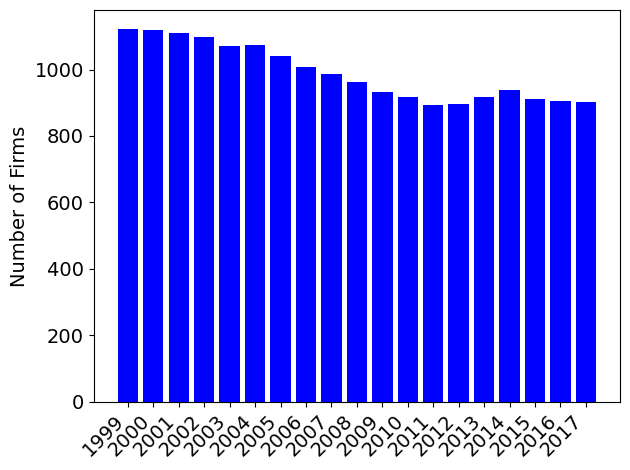
\includegraphics[width=8cm]{figures/number_of_firm}
  \end{center}
\end{frame}

\begin{frame}{Trend of Product Substitutability}
  \begin{center}
    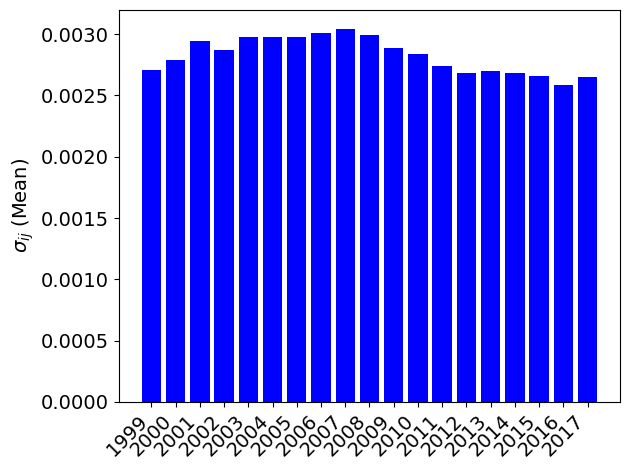
\includegraphics[width=8cm]{figures/sigma}
  \end{center}
\end{frame}

\begin{frame}{Technological Proximity}
  \begin{itemize}
    \item Merge USPTO data with Compustat firms using DISCERN 2 dataset \citep{Arora2024-ad}
    \item Jaffe measure, group-level patent classification, stacked over 5 years
  \end{itemize}
  \begin{center}
    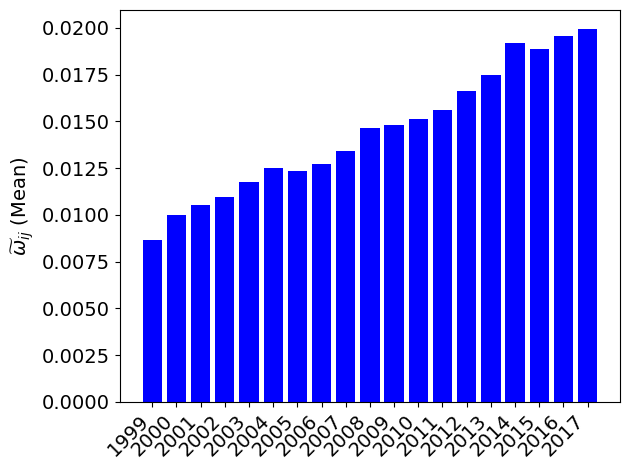
\includegraphics[width=7cm]{figures/omega}
  \end{center}
\end{frame}

\begin{frame}{Correlation Across Networks}
  \label{network_correlations}
  \begin{center}
    \begin{tabular}{lrrr}
      \toprule
               & $K$     & $\Sigma$ & $\Omega$ \\
      \midrule
      $K$      & 1.0000  & -0.0035  & 0.0115   \\
      $\Sigma$ & -0.0035 & 1.0000   & 0.2542   \\
      $\Omega$ & 0.0115  & 0.2542   & 1.0000   \\
      \bottomrule
    \end{tabular}
  \end{center}
  \begin{itemize}
    \item $K$: Ownership network
    \item $\Sigma$: Product substitutability network
    \item $\Omega$: Technological proximity network
  \end{itemize}
  \hyperlink{identification_summary}{\beamerbutton{Back}}
\end{frame}

\begin{frame}[t]{Microeconometric Estimates vs.\ GHL \citep{Pellegrino2024-dn} (1/2)}
  \label{micro_vs_ghl}
  \begin{center}
    \begin{tabular}{lllrr}
      \toprule
      Market & Firm $i$       & Firm $j$       & \multicolumn{1}{c}{Micro Estimate} & \multicolumn{1}{c}{GHL} \\
      \midrule
      Auto   & Ford           & Ford           & -4.320                             & -5.197                  \\
      Auto   & Ford           & General Motors & 0.034                              & 0.056                   \\
      Auto   & Ford           & Toyota         & 0.007                              & 0.017                   \\
      Auto   & General Motors & Ford           & 0.065                              & 0.052                   \\
      Auto   & General Motors & General Motors & -6.433                             & -4.685                  \\
      Auto   & General Motors & Toyota         & 0.008                              & 0.005                   \\
      Auto   & Toyota         & Ford           & 0.018                              & 0.025                   \\
      Auto   & Toyota         & General Motors & 0.008                              & 0.008                   \\
      Auto   & Toyota         & Toyota         & -3.085                             & -4.851                  \\
      \bottomrule
    \end{tabular}
  \end{center}
  \hyperlink{product_identification}{\beamerbutton{Back}}
\end{frame}

\begin{frame}[t]{Microeconometric Estimates vs.\ GHL \citep{Pellegrino2024-dn}  (2/2)}
  \begin{center}
    \begin{tabular}{lllrr}
      \toprule
      Market    & Firm $i$    & Firm $j$    & Micro Estimate & GHL    \\
      \midrule
      Cereals   & Kellogg's   & Kellogg's   & -3.231         & -1.770 \\
      Cereals   & Kellogg's   & Quaker Oats & 0.033          & 0.023  \\
      Cereals   & Quaker Oats & Kellogg's   & 0.046          & 0.031  \\
      Cereals   & Quaker Oats & Quaker Oats & -3.031         & -1.941 \\
      \addlinespace
      Computers & Apple       & Apple       & -11.979        & -8.945 \\
      Computers & Apple       & Dell        & 0.018          & 0.025  \\
      Computers & Dell        & Apple       & 0.027          & 0.047  \\
      Computers & Dell        & Dell        & -5.570         & -5.110 \\
      \bottomrule
    \end{tabular}
  \end{center}
  \hyperlink{product_identification}{\beamerbutton{Back}}
\end{frame}

\begin{frame}{First Stage \hyperlink{regression}{\beamerbutton{Back}}}
  \label{first_stage}
  \begin{center}
    \begin{tabular}{lc}
      \hline
      \hline                          & R\&D \tabularnewline
                                      & (1)\tabularnewline
      \hline
      \begin{tabular}[t]{@{}l@{}}
        State tax credit component \\
        of R\&D user cost
      \end{tabular}   & $\begin{array}{c}
                             -1.16^{***} \\
                             (0.29)
                           \end{array}$\tabularnewline
      \begin{tabular}[t]{@{}l@{}}
        Federal tax credit component \\
        of R\&D user cost
      \end{tabular} & $\begin{array}{c}
                           -34.29^{***} \\
                           (3.64)
                         \end{array}$\tabularnewline
      \hline
      Firm fixed effects              & $\checkmark$\tabularnewline
      Year fixed effects              & $\checkmark$\tabularnewline
      No. of observations             & 16197\tabularnewline
      \hline
    \end{tabular}
    \medskip{}
  \end{center}
  {\footnotesize
  SEs clustered by years and 4-digit NAICS industries are reported in parentheses.
  }
  \medskip{}
  \begin{itemize}
    \item IV: User cost of R\&D, driven by federal and state-specific rules variations \\ \citep{Wilson2009-ri,Bloom2013-pn}
  \end{itemize}
\end{frame}

\begin{frame}{Negative R\&D and Output}
  \label{negative_rd_and_output}
  \begin{itemize}
    \item Issue with the model: negative output and R\&D
          \begin{itemize}
            \item Inada condition is not satisfied
            \item Non-negativity constraint makes model intractable
          \end{itemize}
  \end{itemize}
\end{frame}

\begin{frame}{Negative R\&D and Quantity}
  \begin{itemize}
    \item Firms with negative values are negligible along the transition path
    \item The weight on values 100 years and beyond is 0.005\% when $\rho=0.1$
  \end{itemize}
  \begin{center}
    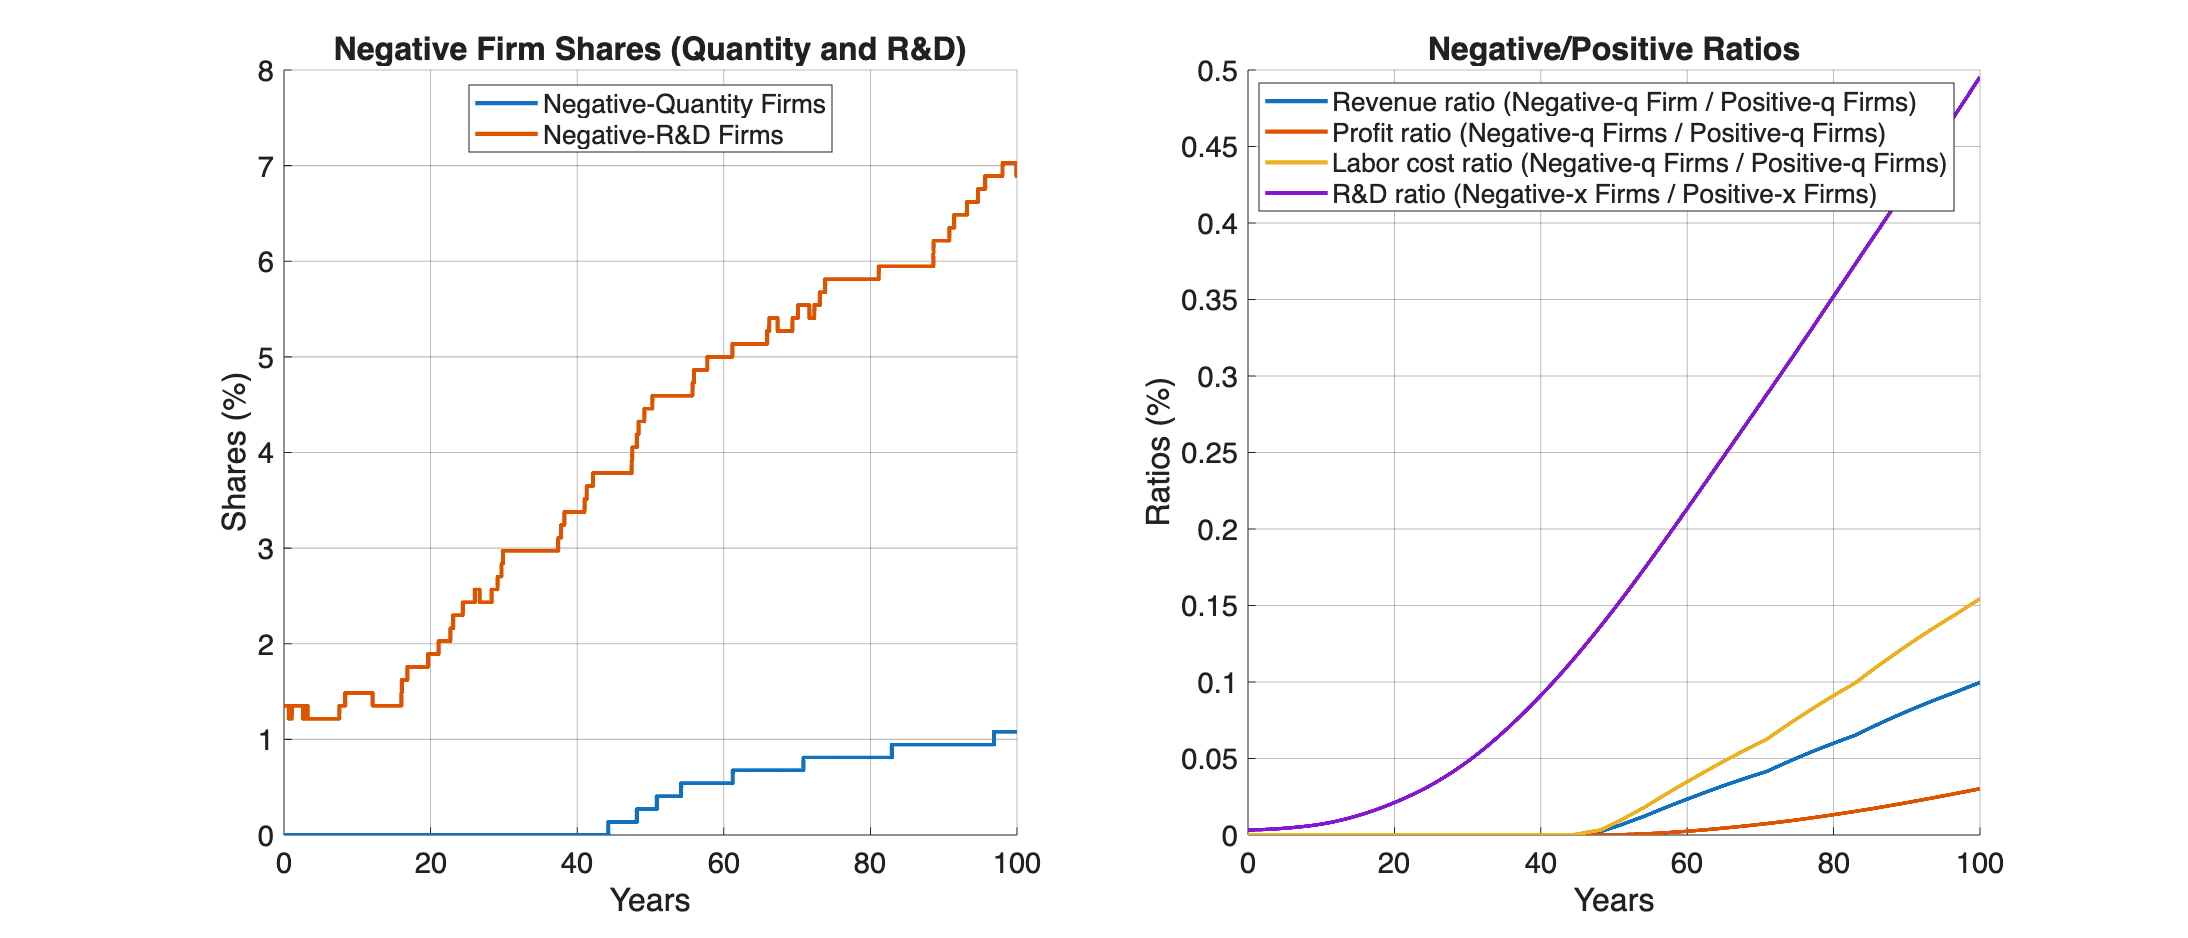
\includegraphics[width=0.8\textwidth]{figures/transition_path_analysis.png}
  \end{center}
  \hyperlink{hjb}{\beamerbutton{Back}}
\end{frame}

\bibliographystyle{econ-aea}
\bibliography{bibtex}

\end{document}
